%This chapter introduces the theoretical foundations on which the proposed learning architecture is built.
The fundamental element of the framework is the tactile skill formalism described in Sec.~\ref{ch:foundations:representation} consisting of the tactile platform, tactile controller, tactile policy, and a performance evaluator.
As a complementary component, a formal process definition is provided that describes industrial processes in terms of manipulation steps and boundary conditions such as error and success states.
In order to connect these two elements, a taxonomy is devised with a hierarchical structure that organizes tactile policies according to process properties.
Based on the tactile skill, process definition, and taxonomy, a synthesis procedure is presented that automatically selects a tactile policy that is suited to solve a given input process.
In Sec.~\ref{ch:foundations:planning} an assembly planner is introduced that makes direct use of the tactile skill concept and extends it to skill sequences. The planner solves the allocation problem for a team of humans and robots for a given assembly problem.
Finally, in Sec.~\ref{ch:foundations:learning} the basis for the learning architecture introduced in Ch.~\ref{ch:architecture} is introduced.
It presents a number of state-of-the-art learning algorithms that are used throughout this thesis as well as useful performance metrics to realize the performance evaluator.
Finally, a robot motor memory effect is described that was discovered in an earlier experiment. The effect forms the basis for the transfer learning experiments described in Ch.~\ref{ch:experiments}.
This chapter was written based on \cite{Johannsmeier.2017,Johannsmeier.2019,Johannsmeier.2023,Johannsmeier.2023b}.
%\section{Taxonomy Verification}\label{ch:experiments:taxonomy}
%In this final section the possible contribution of this thesis to future industrial applications as well as important new research directions are elaborated.

\section{Applications}
\input{chapter/outlook/applications}

\section{Further Research}
\input{chapter/outlook/research}
%\section{Tactile Skill Learning}\label{ch:experiments:learning}
%In this final section the possible contribution of this thesis to future industrial applications as well as important new research directions are elaborated.

\section{Applications}
\input{chapter/outlook/applications}

\section{Further Research}
\input{chapter/outlook/research}
%\section{Performance Comparison: Robot vs. Human}\label{ch:experiments:comparison}
%In this final section the possible contribution of this thesis to future industrial applications as well as important new research directions are elaborated.

\section{Applications}
\input{chapter/outlook/applications}

\section{Further Research}
\input{chapter/outlook/research}
%\section{Collaborative Assembly Planning}\label{ch:experiments:planning}
%In this final section the possible contribution of this thesis to future industrial applications as well as important new research directions are elaborated.

\section{Applications}
\input{chapter/outlook/applications}

\section{Further Research}
\input{chapter/outlook/research}
%\section{Conclusion}\label{ch:experiments:conclusion}
%This chapter describes the extensive experimental work done in this thesis.
Specifically, the taxonomy of manipulation skills is verified with a large number of challenging skills that exhibit high robustness and performance.
This shows that the approach is applicable to a wide range of relevant processes.
The learning architecture is experimentally validated with a number of different learning algorithms and a comparison with state-of-the-art deep learning methods.
The results aid in selecting compatible learning algorithms and show superior results when compared to the state-of-the-art.
Furthermore, a large experimental campaign is described that investigates the architecture’s transfer learning capabilities.
It demonstrates accelerated learning when reusing knowledge to learn new skills and provides insights into the transfer mechanism such as dependency on geometry and asymmetric transferability.
The learning performance as well as achieved manipulation performance were directly compared to human manipulation capabilities and skill programming. The results show that for some skills human performance can already be achieved, while also pointing out the specific gaps that still need to be closed.
Finally, a collaborative assembly problem is solved by an automatic planning system and a human-robot team demonstrating how existing skills can be used automatically to solve even complex tasks.


\section{Introduction}
\subsection{Contributions}
In this paper we cast robot system identification into an incremental learning problem integrating machine learning methods and first-order principles from mechanics and differential geometry. Moreover, we enforce physical conformity of the inertial properties at all times by seamlessly moving on the Riemannian manifold of symmetric positive definite (SPD) matrices, where the inertial parameters of a rigid body are known to reside. We implement a Riemannian gradient descent algorithm with adaptive learning rate and extend it with an experience replay buffer to accelerate convergence and cope with sensor noise. Unlike other approaches, we do not depend on informed initial values. Additionally, we analyze different force/torque measurement setups and evaluate their influence on the learning process. Finally, we implement the method on a real robot and investigate the quality of the inverse dynamics torques generated by the learned parameters and assess the modeling error via a momentum observer.


% ===================================================================================================
%                                                 |                                                 |
%                                                 |                                                 |
% -------------------------------------------- SECTION ---------------------------------------------|
%                                                 |                                                 |
%                                                 |                                                 |
% ===================================================================================================
\section{Literature review}\label{sec:literature_review}


% SUBSECTION ========================================================================================
\subsection{Related works}

\subsubsection{Classical neural networks model learning}
%Conventional neural networks (NN) are often applied to model-learning problems as depicted in Figure~\ref{fig:NN_ID}. The process involves, mainly, the following steps:
Model-learning problems using typical neural networks (NN) involves, mainly, the following steps:
\begin{enumerate}
	\item Input/output data collection: assumed to be available
	\item Architecture design: usually found by trial and error
	\item Parameter optimization/learning: via well understood schemes, e.g., backpropagation and variants
\end{enumerate}
Overall, NN design involves many meta parameters, i.e. number of nodes, numbers of layers, connectivity, activation functions; requiring experts to determine the best topology for a particular problem \cite{Matteucci2006ELeaRNTEvolutionarylearning}. Furthermore, it is difficult to achieve an acceptable level of generalization \cite{Rocha2005Simultaneousevolutionneural}\cite{He2015Topologicaloptimisationartificial}\cite{Matteucci2006ELeaRNTEvolutionarylearning}\cite{Kwok1995Constructivefeedforwardneural}\cite{Lawrence1998Whatsizeneural}\cite{Talebi2010NeuralNetworkBased} as the architecture needs to be balanced to obtain accurate results without overfitting, which may lead to poor generalization, \cite{He2015Topologicaloptimisationartificial}\cite{Muzhou2013NewConstructiveMethod}\cite{Talebi2010NeuralNetworkBased}. Therefore, if a non-parametric model, such as a NN, is used without any model information, large amounts of data are required to generalize to unknown data \cite{Urolagin2012Generalizationcapabilityartificial}.
%\begin{figure}
%    \centering
%    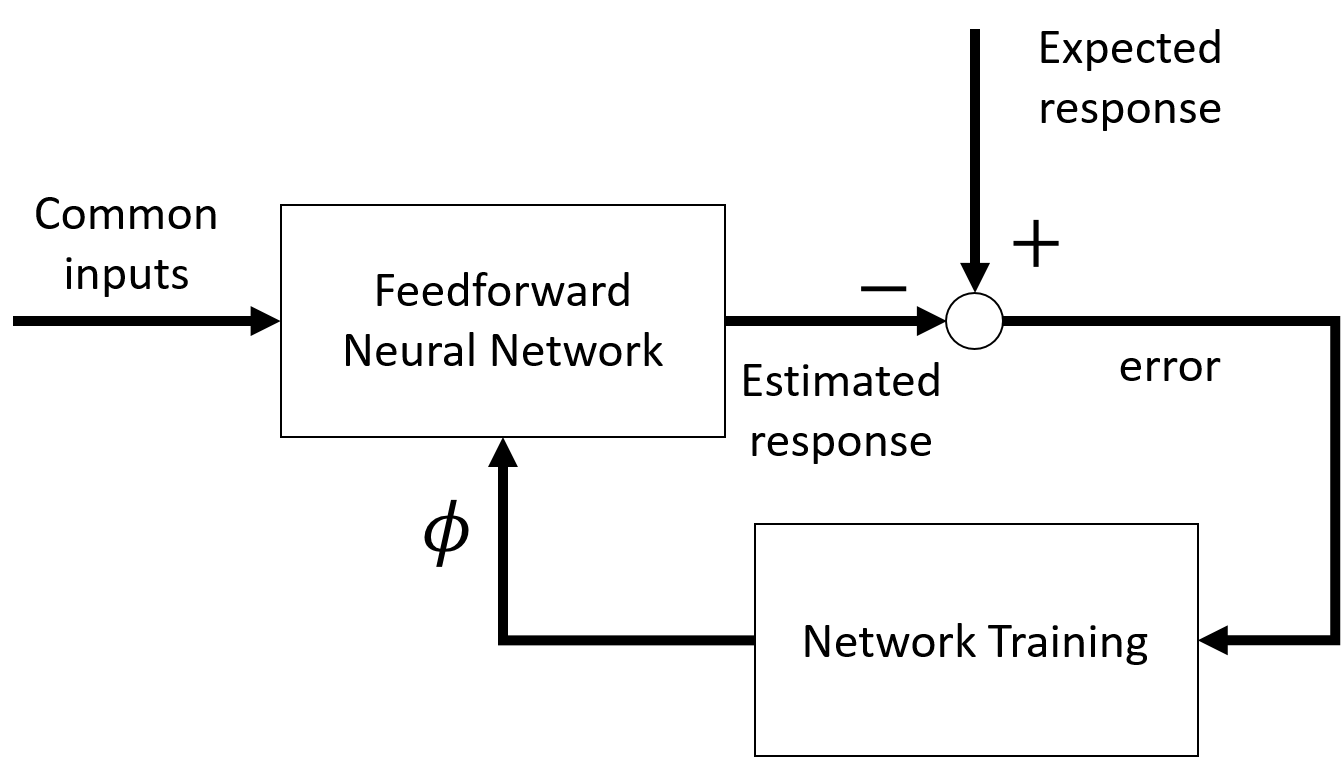
\includegraphics[width=0.3\textwidth]{fig/generalNN_ID}
%    \caption{General model learning using neural networks.}
%    \label{fig:NN_ID}
%\end{figure}

\subsubsection{Topology learning related works}
Finding NN topologies is an important and challenging step \cite{Miikkulainen2017EvolvingDeepNeural}\cite{Rocha2005Simultaneousevolutionneural}\cite{Baker2017Designingneuralnetwork}. Function approximation using NN uses subjective or empirical topologies that are, however, not suitable for interpretation and rely on numerous parameters. As a result, such models are not able to give insight into the actual relation between system variables. 

%As defined in \cite{Matteucci2006}: \textit{"The problem of finding an optimal topology can be thought of as a search problem, where the search space is the space of all possible network topologies, and where the goal is to minimize an error function while preserving generalization capabilities"}. 

Recent works have aimed to find optimal topologies automatically. Evolutionary methods are commonly utilized to optimize the topology and the weights of NN by adding or deleting connections and weights, as shown in \cite{Rocha2005Simultaneousevolutionneural} and \cite{Matteucci2006ELeaRNTEvolutionarylearning} for Feed Forward Neural Networks (FFNN) or \cite{Miikkulainen2017EvolvingDeepNeural} for deep NN. Results tend to show satisfactory generalization capabilities, comparable to human designs. Another method used for FFNN represents the network as a graph and reduces its degrees-of-freedom (DoF), as shown in \cite{He2015Topologicaloptimisationartificial}. Constructive methods are also utilized for FFNN, shown in \cite{Kwok1995Constructivefeedforwardneural}, and pruning methods as applied in \cite{Srinivas2016LearningNeuralNetwork}. Furthermore, reinforcement learning (through Q-learning) and topology learning (using variance analysis) have also been applied to generate the architectures, as shown in \cite{Baker2017Designingneuralnetwork}\cite{Castillo2007Functionalnetworktopology}. Noticeably, for learning complex dynamical systems, such as articulated robot structures, results are still promising, however, limited in accuracy and generalization capabilities \cite{NguyenTuong2011Modellearningrobot}\cite{NguyenTuong2008Learninginversedynamics}\cite{NguyenTuong2010Usingmodelknowledge}. 

\begin{table*}[t]
	\begin{center}
		\begin{tabular}{ |l|l|l|l| } 
			\hline
			&  \textbf{Conventional NN} &  \textbf{FOP Network} & \textbf{Functional Network}\\ 
			\hline
			\textbf{Topology} & Trial \& error & FOP \& system knowledge & System knowledge \\ 
			\hline
			\textbf{Units} & Homogeneous neurons & Parameterized operators & Functions \\ 
			\hline
			\textbf{Activation function} & Sigmoid, tanh, ReLU & Functions & Functions \\   
			\hline
			\textbf{Learned parameters} & Connection weights & Operators parameters \& topology & Neuron function parameters \\
			\hline
			\textbf{Training} & Backpropagation / optimization & Optimization algorithms  & Standard gradient descent and variants\\
			\hline
		\end{tabular}
	\end{center}
	\caption{Comparison between traditional neural networks, first-order principles networks and functional networks.}
	\label{tab:comparison}
\end{table*}


\subsubsection{Robot inverse dynamics estimation via classical NN}\label{sec:classic_inv_dyn}
NN have been applied in numerous variants to model robot inverse dynamics. In \cite{Atencia2015Hopfieldnetworksoptimization}, Hopfield NN were applied to identify the inertial parameters. Moreover, in \cite{Zhu2014Inertiaparameteridentification} a FFNN that used the regressor matrix as training samples was applied. Extreme Learning Machines were utilized in \cite{Bargsten2016ExperimentalRobotInverse} with the same purpose. More recently a two-hidden-layers network with rectified linear activation units (ReLU) was used in \cite{Christiano2016TransferSimulationReal}. Similarly, recurrent NN have been used to account for the sequential nature of the data. \textcolor{red}{In \cite{Yan1997Robotlearningcontrol}, a recurrent NN in the hidden layer of an otherwise conventional three-layer FFNN was proposed.} Additionally, self-organizing-networks, in conjunction with echo state networks, were used in \cite{Polydoros2015Realtimedeep} via a real-time deep learning algorithm.


\subsubsection{Inertial parameters}

Determining the inertial parameters of a robot has been typically achieved using system identification \cite{Atkeson1986Estimationinertialparameters}. Just recently, their physical feasibility has been brought to attention. Works such as \cite{Sousa2014Physicalfeasibilityrobot} study the feasibility conditions on the inertial parameters as convex sets and propose solutions using linear matrix inequalities (LMI). Similarly, authors in \cite{Wensing2017Linearmatrixinequalities} use LMIs to find feasible inertial parameters paying particular attention to the mass distribution. In \cite{Traversaro2016Identificationfullyphysical} \emph{full physical consistency} is introduced and linked to the triangle inequality and the principal moments of inertia of a rigid body. An approach that represents the feasible parameters on the manifold of symmetric positive definite (SPD) matrices is presented in \cite{Lee2018geometricalgorithmrobust}. Extensions to this work within the context of adaptive control are given in \cite{Lee2018naturaladaptivecontrol}. In \cite{Ayusawa2010Identificationstandardinertial}, robot links are represented as a finite number of point masses and use LMIs to introduce physical feasibility constraints. Likewise, \cite{Joukov2015Constraineddynamicparameter} uses an Extended Kalman Filter with sigmoidal constraint functions to estimate online feasible inertial parameters of a robot manipulator. Recently, in \cite{Gaz2019Dynamicidentificationfranka}, system identification of a 7 degrees-of-freedom (DOF) robot was conducted while considering for the first time full physical consistency. None of the methods discussed in these works have considered the problem as an incremental learning problem and only a few have contemplated coupling online learning capability with physical feasibility as a desired feature. As such, their applicability in developmental robotics contexts is hindered. Table \ref{tab:scheme_comparison} contains relevant works with direct focus on full physical feasibility (PF) that are comparable to our work, whether the solution is computed online (OL) or not.

% ===================================================================================================
%                                                 |                                                 |
%                                                 |                                                 |
% -------------------------------------------- SECTION ---------------------------------------------|
%                                                 |                                                 |
%                                                 |                                                 |
% ===================================================================================================
\section{Theoretical framework}\label{sec:theoretical_framework}
A \emph{body schema} is an internal representation of the body, including the arrangement and geometry of its parts, and is built mainly from proprioceptive information \cite{Hoffmann2010Bodyschemarobotics,Morasso2015Revisitingbodyschema}. Adaptive and self-acquired, it is part of an agent's internal forward and inverse models and used to plan and predict sensorimotor interactions. In our view, a robot's body schema encompasses a description of its sensing and actuation capabilities together with its topological, morphological and dynamical characterization. Furthermore, from a developmental perspective, a robot is an embodied agent that autonomously learns and refines incrementally its body schema. Robotics research in this area has focused on discovering the kinematic structure of the robot from exploratory motions and sensorimotor information\cite{Stoytchev2003Computationalmodelextendable, Hart2010RoboticSelfModels, Mathew2014learningbasedapproach, Hoffmann2014Minimallycognitiverobotics, Shoushtari2016Robotbodyself}. Yet, the inertial properties of the agent's body as part of the schema have been neglected. We argue that, in developing a body schema, the robot must incrementally acquire knowledge of these properties to cope with and adapt to alterations in its body. Typically, the classical system identification paradigm has been used to find sets of inertial parameters \cite{Swevers2007Dynamicmodelidentification}; however, it does not contemplate a robot as an embodied agent capable of learning. Alternatively, the machine learning paradigm makes possible the definition of data-driven robot models. Yet, it suffers from a lack of interpretability \cite{Murdoch2019Definitionsmethodsapplications,Rudin2019Stopexplainingblack} and generalization capability limited by the size and variability of the training data. Inspired by both paradigms and starting from knowledge of the robot's kinematic structure, we present a method to incrementally learn the inertial parameters of the robot's constituent links guaranteeing physical feasibility at all times.



% SUBSECTION ========================================================================================


%% ---
%\begin{table*}[!ht]
%	\caption{Research on fully physically consistent inertial parameter learning.}
%	\vspace{-2ex}
%	\begin{center}
%		\resizebox{\textwidth}{!}{%
%			\begin{tabular}{|c|x{5cm}|x{5cm}|c|c|} 
%				\hline
%				\textbf{Study} &  \textbf{Key concept} &  \textbf{Solution method} &  \textbf{OL} & \textbf{PF} \\ 
%				
%				\hline
%				\citeauthor*{Sousa2019Inertiatensorproperties} (\citeyear{Sousa2019Inertiatensorproperties})\cite{Sousa2019Inertiatensorproperties}	  & Feasibility of base parameters & Linear Matrix Inequalities - Semidefinite Programming & \xmark & \Checkmark 
%				\\		
%				
%				\hline
%				\citeauthor*{Traversaro2016Identificationfullyphysical}
%				(\citeyear{Traversaro2016Identificationfullyphysical})\cite{Traversaro2016Identificationfullyphysical} & Full physically consistent parametrization & Nonlinear optimization on manifolds & \xmark & \Checkmark
%				\\
%				
%				\hline
%				\citeauthor*{Wensing2017Linearmatrixinequalities} (\citeyear{Wensing2017Linearmatrixinequalities})\cite{Wensing2017Linearmatrixinequalities} & Manifold parameterization of full physical consistency & Linear Matrix Inequalities - Semidefinite Programming & \xmark & \Checkmark
%				\\
%				
%				\hline
%				\rowcolor{Gray}
%				\citeauthor*{Lee2018naturaladaptivecontrol} (\citeyear{Lee2018naturaladaptivecontrol})\cite{Lee2018naturaladaptivecontrol} & Natural adaptive control law based on SPD manifold & Natural gradient descent & \textcolor{black}{\Checkmark} & \textcolor{black}{\Checkmark}
%				\\
%		\end{tabular}}
%	\end{center}
%	\label{tab:scheme_comparison}
%\end{table*}
%% ---

% ===================================================================================================
%                                                 |                                                 |
%                                                 |                                                 |
% -------------------------------------------- SECTION ---------------------------------------------|
%                                                 |                                                 |
%                                                 |                                                 |
% ===================================================================================================
\subsection{Learning the inertial parameters in the SPD manifold}\label{sec:rb_ip_on_spd}

% SUBSECTION ========================================================================================
\subsubsection{The space of symmetric positive definite matrices}\label{sec:spd_manifold}
A \emph{differentiable manifold} $\mathcal{M}$ is a topological space that is locally similar to Euclidean space and has a globally defined differential structure \cite{Jayasumana2013KernelmethodsRiemannian}. $\mathcal{T}_{\bm{P}}\mathcal{M}$ is the \emph{tangent space} at a point $\bm{P}\in \mathcal{M}$ and represents the vector space of all the possible tangent vectors to the manifold that pass through $\bm{P}$. The pair $(\mathcal{M},\rho)$ defines a \emph{Riemannian manifold} if $ \mathcal{M} $ is differentiable and is equipped with a positive definite metric tensor $\rho$ at each point \cite{Pennec2006Riemannianframeworktensor}. 

Let $\mathcal{S}^n \triangleq\left\lbrace \bm{S} \in \mathbb{R}^{n \times n} : \bm{S} = \bm{S}^T\right\rbrace$ be the space of real square symmetric matrices of dimension $n \times n$. Then, the space of $n \times n$ SPD matrices $ \mathcal{S}^n_{++}\triangleq \left\lbrace \bm{P}\in \mathcal{S}^n : \bm{P} \succ 0 \right\rbrace $  defines a smooth submanifold $\mathcal{M}$ of $\mathcal{S}^n$. By definition, its tangent space $\mathcal{T}\mathcal{M} \in \mathcal{S}^n$ is equipped with an \emph{affine invariant Riemannian metric} $\rho$ \cite{Lee2018geometricalgorithmrobust}. Consequently, $ \mathcal{S}^n_{++} $ defines a Riemannian manifold. Finally, the product manifold $ \mathcal{M}^N $ of SPD manifolds is the Cartesian product $\mathcal{M}^N =\mathcal{M}_1\times \mathcal{M}_2\times \ldots \times \mathcal{M}_N$. It is the set of matrices  $\left\lbrace \left(\bm{P}_1,\ldots,\bm{P}_N\right):\bm{P}_i\in\mathcal{M}_i,\quad i=1,\ldots,N\right\rbrace$ and is also a Riemannian manifold with the metric $ \bm{\rho} =\text{diag}\left( \rho_{1},\ldots, \rho_{N} \right) $. Similarly, the generalizations of the operators mentioned above to $\mathcal{M}^N$ are the concatenations of the individual operators for each $\mathcal{M}_i$.

% SUBSECTION ========================================================================================
\subsection{The inverse dynamics problem}
Let $ \bm{w} = \bm{W}\left(\bm{q},\dot{\bm{q}},\ddot{\bm{q}}\right)\bm{\theta} $ denote the inverse dynamics equation of a serial robot with $N$ links, where the inputs are the vector of joint angles $ \bm{q} $ and its first and second derivatives. We use here the formulation $ \bm{w} = \bm{W}\left(\bm{\omega},\dot{\bm{\omega}},\dot{\bm{v}}\right)\bm{\theta} $ as it allows the decoupling of the kinematics and dynamics parts of the robot model \cite{DiazLedezma2018FOPNetworksLearning}. The vector $\bm{w} = [\bm{w}^T_1,\cdots, \bm{w}^T_N]^T$ contains the wrenches of all the bodies in the kinematic chain expressed in the corresponding body frame. Each wrench is composed of the forces $\bm{f}_i$ and moments $\bm{n}_i$ acting on the $ i $-th body, e.g. $\bm{w}_i = \left[\bm{f}_i^T, \bm{n}_i^T \right]^T$. The regressor matrix $\bm{W}(\cdot)$ depends on the robot kinematics and the Cartesian angular velocities $\bm{\omega}_i$, as well as on the angular $\dot{\bm{\omega}}$ and linear accelerations $\dot{\bm{v}}$\footnote{It is worth mentioning that the vector $\bm{w}$ and, correspondingly, the matrix $\bm{W}$ can be adjusted according to the available sensors.}.
The vector $ \bm{\theta}=\begin{bmatrix} \bm{\theta}_1^\intercal & \ldots  & \bm{\theta}_i^\intercal & \ldots & \bm{\theta}_N^\intercal \end{bmatrix}^\intercal  $ contains the inertial parameters of the robot, with $ \bm{\theta}_i = [\begin{smallmatrix} m_i & \bm{h}^\intercal_i & XX_i & XY_i & XZ_i & YY_i & YZ_i & ZZ_i \end{smallmatrix}]^T \in \mathbb{R}^{10} $ and $ \bm{h}_i =
\begin{bmatrix} mX_i & mY_i & mZ_i\end{bmatrix}^T $. The first element of $\bm{\theta}_i$ is the mass of link $i$, the vector $\bm{h}_i$ contains the first moments of mass, and the last six entries are the elements of the inertia matrix of link $i$ expressed in joint frame $i$.

%% SUBSECTION ========================================================================================
%\subsection{Physical feasibility of the inertial parameters}
%The constraints that ensure fully physically feasible $\bm{\theta}_i$ are a strictly positive mass and a SPD inertia matrix $ \bm{I}_i $ with its eigenvalues ---$\lambda\left(\bm{I}_i\right) = [\lambda_1,\lambda_2,\lambda_3]^T$--- satisfying the triangle inequality, i.e.:\\
%%---
%\begin{equation}\label{eq:feasibility_constraints}
%	m_i>0, 
%	\quad
%	\resizebox{0.4\hsize}{!}{$
%		\bm{I}_i=\begin{bmatrix}
%			XX_i & XY_i & XZ_i \\ XY_i & YY_i & YZ_i\\ XZ_i& YZ_i & ZZ_i
%		\end{bmatrix} \succ 0$},
%	\quad
%	\begin{aligned}
%		\resizebox{0.25\hsize}{!}{$\begin{cases}
%				\lambda_1 + \lambda_2 \geq \lambda_3\\
%				\lambda_2 + \lambda_3 \geq \lambda_1\\
%				\lambda_1 + \lambda_3 \geq \lambda_2
%			\end{cases}$}
%	\end{aligned} 
%\end{equation}
%%---
%Moreover, physical feasibility is achieved as long as the symmetric $4 \times 4$ \emph{pseudo inertia matrix}
%%---
%\begin{equation}\label{eq:pseudo_inertia_matrix}
%	\bm{P}_i(\bm{\theta}_i)=f(\bm{\theta}_i)=\begin{bmatrix}
%		\bm{\Sigma}_i && \bm{h} \\ \bm{h}^T && m
%	\end{bmatrix}\in \mathcal{S}^4,
%\end{equation}
%%---
%defined for each rigid body is positive-definite \cite{Wensing2017Linearmatrixinequalities}. Here $ \bm{\Sigma}_i = \frac{1}{2}\Tr(\bm{I}_i)\mathbb{1} - \bm{I}_i\in \mathcal{S}^3 $ is called the \emph{density weighted covariance matrix}. Conversely,  $ \bm{I}_i = \Tr\left(\bm{\Sigma}_i\right)\mathbb{1} - \bm{\Sigma}_i \in \mathcal{S}^3_{++} $, where $\mathbb{1}$ is the $3 \times 3$ identity matrix. The requirement that $\bm{P}_i(\bm{\theta}_i) \succ 0$ implies the fully physically feasible inertial parameters are in the manifold $\mathcal{S}^4_{++}=\left\lbrace \bm{P}_i(\bm{\theta}_i) \in \mathcal{S}^{4}: \bm{P}_i(\bm{\theta}_i) \succ 0 \right\rbrace$. As explained in \cite{Lee2018geometricalgorithmrobust}, for every rigid body $i$ in the kinematic chain, there exist a pseudo inertia matrix \eqref{eq:pseudo_inertia_matrix}. This means that the set of matrices  $\left\lbrace \bm{P}_i\right\rbrace_{i=1}^N$ resides in $\mathcal{M}^N$.
%
%% SUBSECTION ========================================================================================
%\subsection{Online learning of the inertial parameters}
%Let $\bm{w}_k$ and $\hat{\bm{w}}_k(\hat{\bm{\theta}})$ be the measured and estimated joint wrench at time $k$. The optimal fully-physically-feasible estimated inertial parameters $ \hat{\bm{\theta}} $ minimize the mean squared error $ J(\cdot) $ for a recurrently-updated mini batch of $ N_{\mathcal{X}} $ samples while satisfying the constraints $\mathcal{\Theta}$ given in %\eqref{eq:positive_mass}, \eqref{eq:spd_inertia}, \eqref{eq:triangular_inequalities}. 
%\eqref{eq:feasibility_constraints}. Learning $ \hat{\bm{\theta}} $ online requires starting from an initial guess $\hat{\bm{\theta}}_0$ collecting input-output pairs $ \left(\bm{x}_k, \bm{w}_k\right)  $ on-the-fly generated by the robot's motion, with $ \bm{x} = \left[\bm{q}^T,\bm{\omega}^T,\dot{\bm{\omega}}^T,\dot{\bm{v}}^T\right]^T $, and then updating $ \hat{\bm{\theta}} $ at every time step $ k $ based on the incoming data and the metric  $J(\cdot) $. However, incorporating the constraints $\mathcal{\Theta}$ to the online setting is challenging due to their nonlinearity. 
%
%% ===================================================================================================
%%                                                 |                                                 |
%%                                                 |                                                 |
%% -------------------------------------------- SECTION ---------------------------------------------|
%%                                                 |                                                 |
%%                                                 |                                                 |
%% ===================================================================================================
%\section{Riemannian Incremental Learning}\label{sec:riemannian_opt}
%% SUBSECTION ========================================================================================
%\subsection{General description}
%To circumvent the need for $\mathcal{\Theta}$, in this work we translate the Euclidean learning problem from
%\begin{equation}\label{eq:dyn_cost_func_euclidean}
%	%	\underbrace{
%		\begin{aligned}
%			& \underset{\hat{\bm{\theta}}}{\text{min}}
%			& &J(\hat{\bm{\theta}})=\frac{1}{2N_{\mathcal{X}}}\sum_{k=1}^{N_{\mathcal{X}}} \left\lVert \bm{w}_k-\hat{\bm{w}}_k(\hat{\bm{\theta}}) \right\rVert^2_2\\
%			& \text{subject to}
%			& & \hat{\bm{\theta}} \in \Theta
%		\end{aligned}
%		%	}_{Constrained}
%\end{equation}
%to
%\begin{equation}\label{eq:dyn_cost_func_manifold}
%	\underbrace{
%		\begin{aligned}
%			& \underset{\hat{\bm{P}}\in \mathcal{M}^N}{\text{min}}
%			& &J(\hat{\bm{P}})=\frac{1}{2N_{\mathcal{X}}}\sum_{k=1}^{N_{\mathcal{X}}} \left\lVert \bm{w}_k-\hat{\bm{w}}_k(\hat{\bm{P}}) \right\rVert^2_2,
%	\end{aligned}}_{Unconstrained}
%\end{equation}
%%---
%such that all constraints are inherently met by requiring $ \hat{\bm{\theta}} \in \mathcal{M}^N$, and update $ \hat{\bm{\theta}} $ according to Algorithm~\ref{alg:rams_gd}. We call the method \emph{Riemannian Incremental Learning} (RIL), as it is tailored for online learning and is based on Riemannian updates. An overview of RIL is shown in Fig.~\ref{fig:riemannian_incremental_learning}. Based on a developmental approach, it assumes no prior knowledge of the inertial properties and incrementally learns them based on gathered experience from exploration motions. Such motions result from the \emph{Excitation Motion Generator}\footnote{The online generation of excitation trajectories is not the focus of this paper and remains an open problem that we will tackle in subsequent work.} \textcircled{1} (not considered here) and are driven by a pure \emph{Feedback Controller} \textcircled{2} as no model is yet available. The torques given to the robot and the signals from joint position velocity and acceleration are fed to block \textcircled{5} to compute \emph{Riemannian Updates} to the estimated inertial parameters $ \hat{\bm{\theta}} $ using Algorithm~\ref{alg:rams_gd} and a Newton-Euler-derived regressor matrix from the \emph{Model} block \textcircled{4}. As time progresses these estimates are refined and at a time $ t=T_{s} $, determined by a convergence criterion, the model is ready to provide the inverse dynamics torques $ \bm{\tau}_{RIL} $ generated by the $ \hat{\bm{\theta}} $-parameterized model.
%---
\begin{figure}[t!]
	\centering
	\hspace*{\fill}
	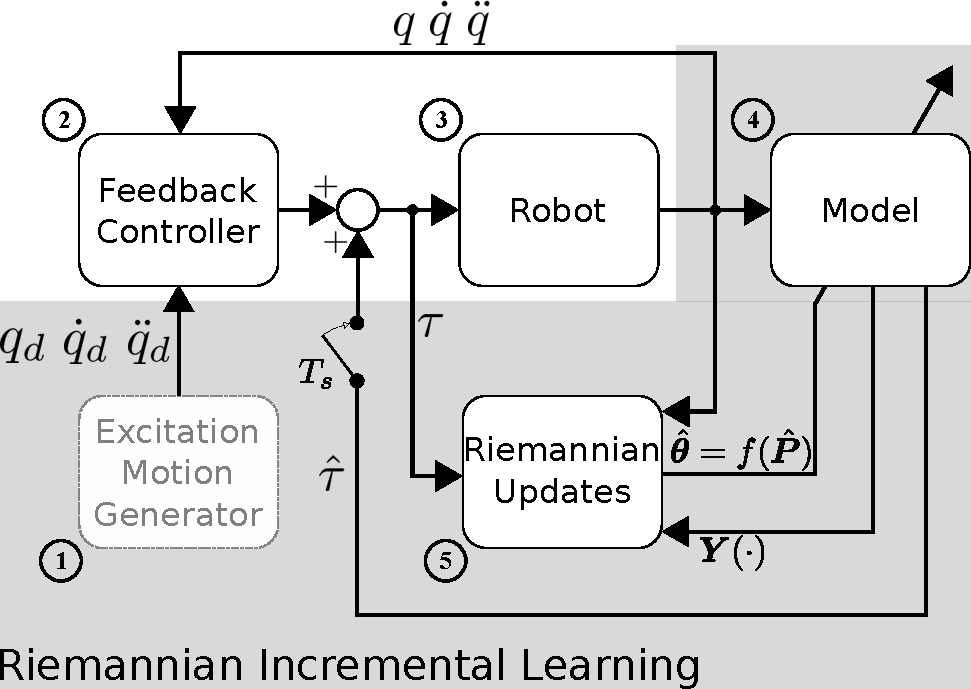
\includegraphics[width= 0.7\columnwidth]{riemannian_incremental_learning.pdf} 
	\hspace*{\fill}
	\caption[] {Overview of the proposed learning scheme.}\label{fig:riemannian_incremental_learning}
\end{figure}
%--- 
%% SUBSECTION ========================================================================================
%\subsection{Riemannian gradient descent on $ \mathcal{S}^{4}_{++} $}
%The \emph{Riemannian gradient} at a point $\bm{P}\in\mathcal{M}$ is the orthogonal projection of the gradient in ambient Euclidean space $\bm{G} = \nabla J(\cdot)=\frac{\partial J}{\partial \bm{P}}\in \mathbb{R}^{n \times n}$ onto $\mathcal{T}_{\bm{P}}\mathcal{M}$ \cite{Boumal2014Optimizationestimationmanifolds.}; that is, 
%$ \text{grad}_{\bm{P}}J(\bm{P}) = \Pi_{ \mathcal{T}_{\bm{P}}}\left(\nabla J(\bm{P})\right) \in \mathcal{T}_{\bm{P}}\mathcal{M} $, with the projection operator defined as $\Pi_{ \mathcal{T}_{\bm{P}}}(\bm{G})\triangleq\bm{P}\left(\frac{\bm{G}+\bm{G}^T}{2}\right)\bm{P},\quad \forall \bm{P}\in \mathcal{M}  $ \cite{Brooks2019Riemannianbatchnormalization}. As described in \cite{Bonnabel2013Stochasticgradientdescent}, Riemannian gradient descent uses $
%\bm{P}^{k+1}= \text{Exp}_{\bm{P}^k}\left(-\gamma \text{grad}_{\bm{P}^k}J(\bm{P}^k)\right)$, $ \gamma \in (0,1]$, to compute the update to the parameter $\bm{P}$ on $\mathcal{M}$. Likewise, the Riemannian gradient of a function $J(\bm{P})$ at a point $\bm{P}=(\bm{P}_1,\ldots,\bm{P}_N)\in\mathcal{M}^N$ is expressed by $
%\text{grad}_{\bm{P}}J=\left(\text{grad}_{\bm{P}_i}J_1, \ldots, \text{grad}_{\bm{P}_N}J_N\right)$;  with $\bm{P}_i\in\mathcal{M}_i$, i.e. defined on a product manifold.
%%
%Here the term $\text{grad}_{\bm{P}_i}J_i$ represents the Riemannian gradient of the partial map $
%J_i:\bm{Q}\in \mathcal{M}_i \mapsto f\left(\bm{P}_1,\ldots,\bm{P}_{i-1},\bm{Q},\bm{P}_{i+1},\ldots,\bm{P}_N\right)$. 
%%---
%\begin{center}
%	\begin{algorithm}[t!]\small
%		\caption{RAMS gradient descent in $\mathcal{M}^N$}\label{alg:rams_gd}
%		\begin{algorithmic}[1]
%			%		\Procedure{Parameter update}{$n$}
%			\State \textbf{Require} $\hat{\bm{P}}(0)\in \mathcal{S}^4_{++}$ initial feasible point
%			\State \textbf{Require} $\beta_1,~\beta_2 \in \left[0,1\right)$ exponential decay rates for moment estimates%\footnote{The standard values for the first momentum term $ \beta = 0.9 $ and second momentum term $ \beta_2 = 0.999 $ are considered.}
%			\State \textbf{Require} $\alpha$~learning rate
%			\State $\bm{P}_t \gets \hat{\bm{P}}(0)$~\Comment{initialization}
%			\State $\bm{m}_t \gets \bm{0}$
%			\State $\bm{\tau}_t \gets \bm{0}$
%			\State $v_t \gets 0$
%			\State $\hat{v}_t \gets 0$
%			\For{$t= 1$ to $T_s$} \Comment{loop over samples}
%			\State $\mathcal{B} \gets  \bm{x}_t $ \Comment{store current sample}
%			%\tikzmark{top}
%			\State Select $ \mathcal{X} $  from $ \mathcal{B} $
%			% \tikzmark{right}
%			\State Compute $ J(\bm{P}\lvert\ \mathcal{X}) $ and $ \text{grad}_{\bm{P}_t}J(\cdot) $					
%			\For{$i=1$ to N} 
%			%\tikzmark{bottom}
%			\State $ \bm{g}^i_t = \text{grad}_{\bm{P}_t}J_i(\bm{P}_t\lvert\ \mathcal{X}) $
%			\State $ \bm{m}^i_t = \beta_1 \bm{\tau}^i_{t-1} + (1 - \beta_1)\bm{g}^i_t $
%			\State $ v^i_t = \beta_2 v^i_{t-1} + (1 - \beta_2) \left\lVert \bm{\bm{g}^i_t} \right\rVert^2_{\bm{P}_t} $
%			\State $ \hat{v}^i_t = \text{max}(\hat{v}^i_{t-1},v^i_t)  $
%			\State $ \bm{P}^i_{t+1}= \text{Exp}^i_{\bm{P}^i_t}\left(- \frac{\alpha}{\sqrt{\hat{\bm{v}}^i_t + \epsilon}}\bm{m}^i_t\right) $
%			\State 	$ \bm{\tau}^i_t = \Gamma^i_{\bm{P}^i_t\to \bm{P}^i_{t+1}}\left(\bm{m}^i_t\right) $
%			\EndFor
%			\EndFor
%			\State \textbf{return} $\bm{P}^i_{t+1}$ for $i=1,\ldots,N$ \Comment{parameter updates}
%		\end{algorithmic}
%		%			\AddNote{top}{bottom}{right}{Replay buffer.}
%	\end{algorithm}
%\end{center}
%%---
%Motivated by the stability and convergence speed of the state-of-the-art online gradient descent algorithm AMSGrad \cite{Reddi2019convergenceADAM}, we now use its manifold version, the Riemannian AMS gradient descent ---RAMSGrad for short \cite{Becigneul2018Riemannianadaptiveoptimization}. \textcolor{black}{Algorithm~\ref{alg:rams_gd} shows the core steps of RAMSGrad, where $ \bm{m}_t $ and $ v_t $ are the moving averages of the gradient and its Riemannian norm. The term $ \bm{\tau}_t $ allows the aggregation of the previous gradients by considering the curvature of the manifold. 	Finally, $ \alpha $ is the initial learning rate. In our implementation, the standard values for the first and second momentum terms are used ($ \beta_1 = 0.9 $, $ \beta_2 = 0.999 $). The algorithm runs up to a final user-defined time $ T_s$. We expand the algorithm introducing an experience replay buffer $ \mathcal{B} $ to break the correlation between consecutive samples by storing $N_{\mathcal{B}}$ previous data points. At every time step $ t $ the current sample $ \bm{x}_t $ is pushed into the buffer by taking the place of a randomly-chosen sample. From $ \mathcal{B} $ a mini batch $ \mathcal{X} $ of $ N_{\mathcal{X}}  $ samples is selected and used to compute the cost $ J(\bm{P}_t \lvert\ \mathcal{X}) $ and its corresponding Riemannian gradient $
%	\text{grad}_{\bm{P}}J$. %This mitigates the temporal correlations of the samples and induces a more \emph{independent and identically distributed} construction of the mini batches.}
%This results in mini batches constructed from \emph{independent and identically distributed} samples with no temporal correlation.}
%
%% ===================================================================================================
%%                                                 |                                                 |
%%                                                 |                                                 |
%% -------------------------------------------- SECTION ---------------------------------------------|
%%                                                 |                                                 |
%%                                                 |                                                 |
%% ===================================================================================================
%\section{Results}
%% SUBSECTION ========================================================================================
%\subsection{Influence of force/torque measurement setups}
%Using a virtual robot with fully determined properties we analyze the influence of different joint force/torque measurement setups on the $ \hat{\bm{\theta}} $ generated by RIL. The robot is made of cylindrical bodies of uniform density and revolute joints that rotate around the z-axis of the corresponding joint frame. Fig.~\ref{fig:cylindrical_robot} shows the structure of the robot together with the actual inertia ellipsoids for all its links. To generate motion data, a set of pre-computed excitation trajectories was given to the manipulator and the joint wrenches were computed using the recursive Newton-Euler algorithm. RIL was used to generate Riemannian updates based on \eqref{eq:dyn_cost_func_manifold} and starting from $ {\hat{\bm{P}}_i(0)}_{i=1}^N = \bm{I}_{4\times4}$ (identity matrix), i.e. \textbf{prior information is neither used nor required}. Additionally, we set the replay buffer $ \mathcal{B} $ to  hold $ N_{\mathcal{B}} =5$ samples and a mini batch $ \mathcal{X} $ with size equal to the buffer size. We contemplate three different force/torque measurement setups as supervisory signals: (a) joint wrench, (b) wrench at the first joint and all subsequent joint torques, and (c) only joint torques. Figure~\ref{fig:cylindric_robot_estimated_structure} shows the resulting inertia ellipsoids for each setup. Clearly, wrench measurements (see Fig.~\ref{fig:cylindrical_robot_wrench}) lead to parameters that closely resemble ground truth. In contrast, with joint torques only, it is not possible to fully reproduce the original set, as seen noticeably by the wanting estimations of the proximal links. Nonetheless, estimates for the distal-most links do approximate the real values. Finally, the information provided by a force/torque sensor at the first joint results in improvements to the location of the center of mass of the proximal links, see  Fig.~\ref{fig:cylindrical_robot_wrenchTorque}. To the right of Figs.~\ref{fig:cylindrical_robot_wrench} to \ref{fig:cylindrical_robot_wrenchTorque}, the results of learning when choosing $ \hat{\bm{P}}(0) = \bm{P}^*(1 + \bm{\epsilon})$, where  $ \bm{P}^* $ are the actual values and $ \bm{\epsilon} \sim \mathcal{N}(0,0.5)$ is a small perturbation, are displayed. This shows that, when the initial values are in the vicinity of the real values, RIL will induce negligible changes.
%%---
%\begin{figure}
%\centering	
%\hspace*{\fill}
%\subfloat[]{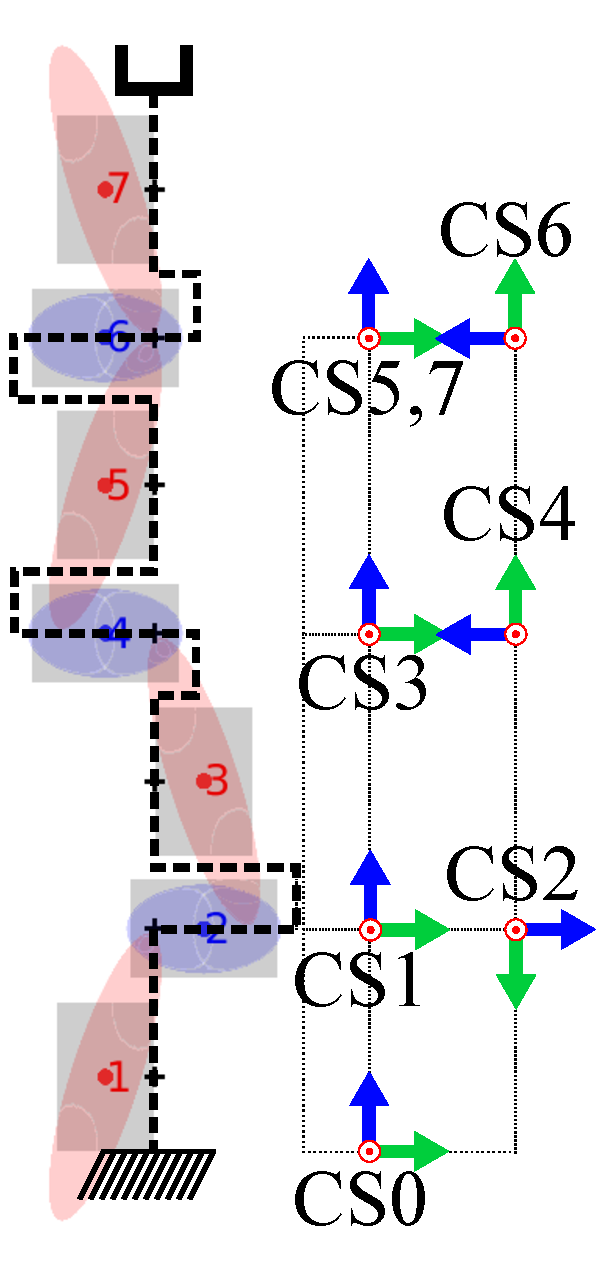
\includegraphics[width= 0.23\columnwidth]{fig/cylindrical_robot_update.pdf} \label{fig:cylindrical_robot}}
%\hspace*{-0.9em}
%\subfloat[]{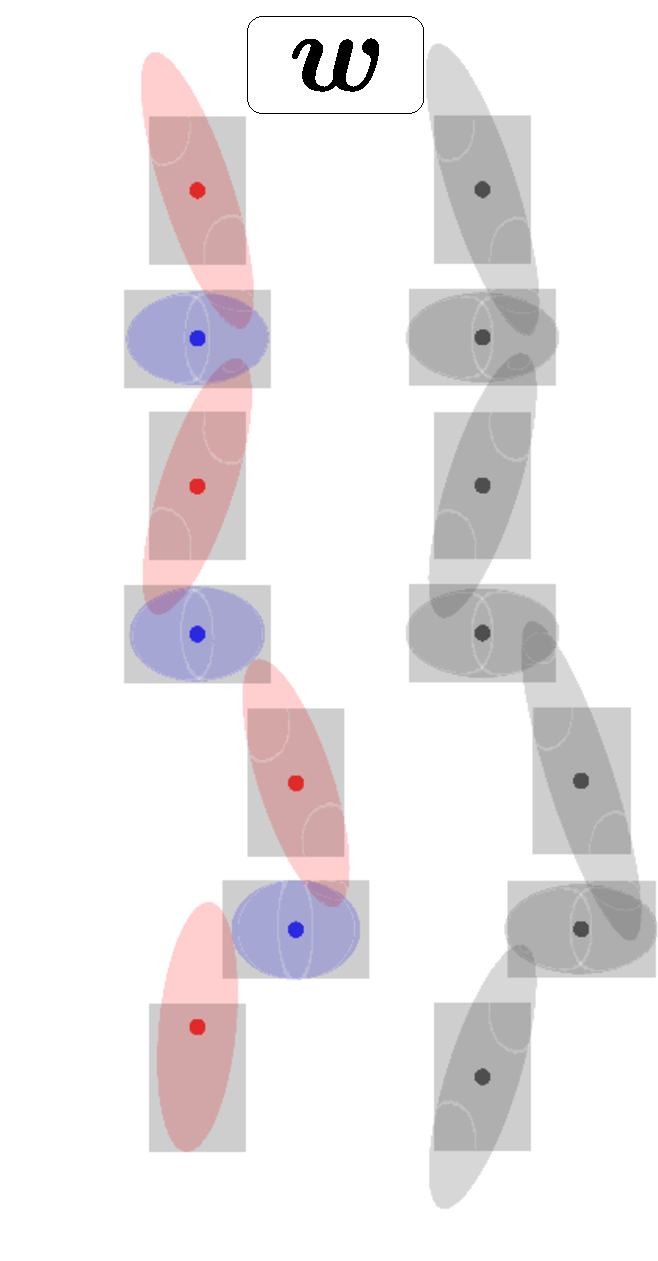
\includegraphics[width= 0.25\columnwidth]{fig/cylbot_wrench_v2.pdf} \label{fig:cylindrical_robot_wrench}}
%\hspace*{-0.9em}
%\subfloat[]{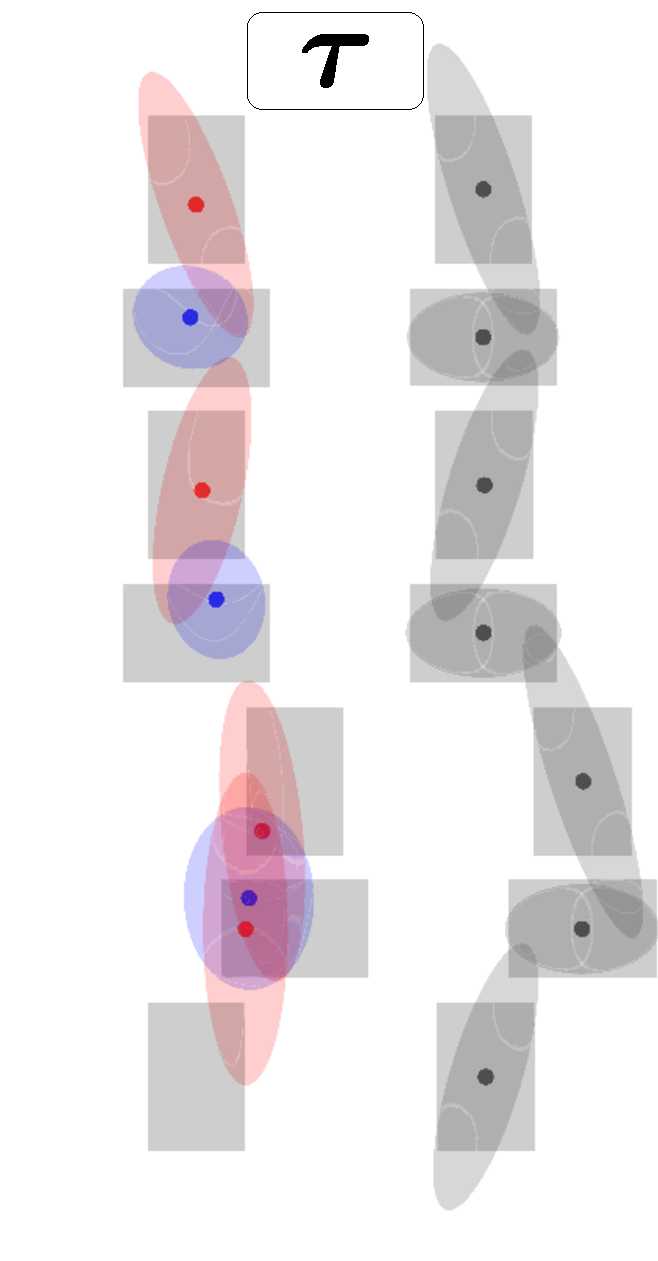
\includegraphics[width= 0.25\columnwidth]{fig/cylbot_torque_v2.pdf} \label{fig:cylindrical_robot_torque}}
%\hspace*{-0.9em}
%\subfloat[]{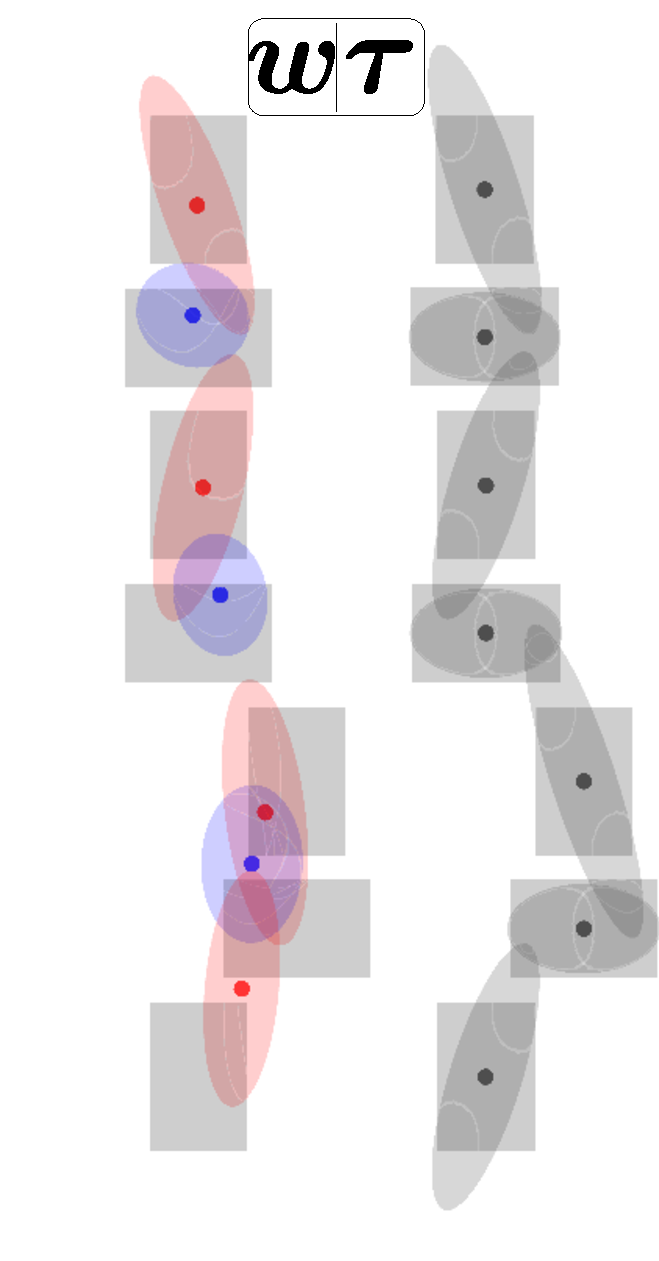
\includegraphics[width= 0.25\columnwidth]{fig/cylbot_wrench_torque_v2.pdf} \label{fig:cylindrical_robot_wrenchTorque}}			
%\hspace*{\fill}
%\caption[] {\label{fig:cylindric_robot_estimated_structure} A robot with cylindrical links and their corresponding inertial ellipsoids: \subref{fig:cylindrical_robot} actual structure, estimation using \subref{fig:cylindrical_robot_wrench} joint wrench ($ \bm{w} $), \subref{fig:cylindrical_robot_torque} joint torque only ($ \bm{\tau} $), \subref{fig:cylindrical_robot_wrenchTorque} first joint wrench and the torques from subsequent joints ($ \bm{w}|\bm{\tau} $).}
%\end{figure}
%%---
%% SUBSECTION ========================================================================================
%\subsection{Simulated Franka Emika Panda}
%Now we consider a model of a state-of-the-art 7 DoF collaborative robot, the Franka Emika Panda. For this we take as ground truth the inertial parameters reported in \cite{Gaz2019Dynamicidentificationfranka}, found using classical system identification (SID), and use the Newton-Euler approach to simulate the forward and inverse dynamics of the robot.  In the experiment the manipulator executes repeatedly a series of pre-computed excitation trajectories composed of the sum of a Fourier series and a polynomial, as described in \cite{Park2006Fourierbasedoptimal}. Additionally, the end-effector holds a load to generate significant joint torques at the distal joints.  RIL is then used to learn the parameters and evaluate how they compare to the values reported in \cite{Gaz2019Dynamicidentificationfranka}. This time we set $ N_{\mathcal{B}}=$1000 for the replay buffer. 
%% ---------------------------------------------------------------------------------------------------
%\subsubsection{Change in load}
%To evaluate if RIL can adapt to structural changes an experiment was performed in which the test load ($ m_L = \unit[1.45]{kg} $) was learned as part of the manipulator's body and was then suddenly removed. This resembles an abrupt change in the dynamic properties. The experiment allowed us to see how fast RIL can adapt to such changes. The test ran for 1000 seconds with the load being removed at $ t = \unit[700]{s} $. Fig.~\ref{fig:load_drop_mass_estimates} shows the estimates from RIL for all the masses. We chose to focus on the link masses to address one potential limitation: the dependence on proprioception. Taking the seventh link's mass as example ($m_7 = \unit[1.46]{kg} $), it can be seen that while the load is held, the estimation of the compound mass is reasonably good; i.e. $ \hat{m}_7 \simeq m_7 + m_L $. When the load is removed, a large difference between the actual mass and the estimated mass is evident ($\hat{m}_7< \unit[1]{kg}$). Although the learning metric $ J(\cdot) $ is still minimized, it obviously deviates from reality. The cause of this is that RIL depends on proprioceptive information, i.e. joint measurements. In particular, without a test load, the torque at the seventh joint is considerably small in relation to the rest, a fact that naturally complicates the correct learning of the 7th link parameters.
%%---
%\begin{figure}[t!]
%\centering
%\hspace*{\fill}
%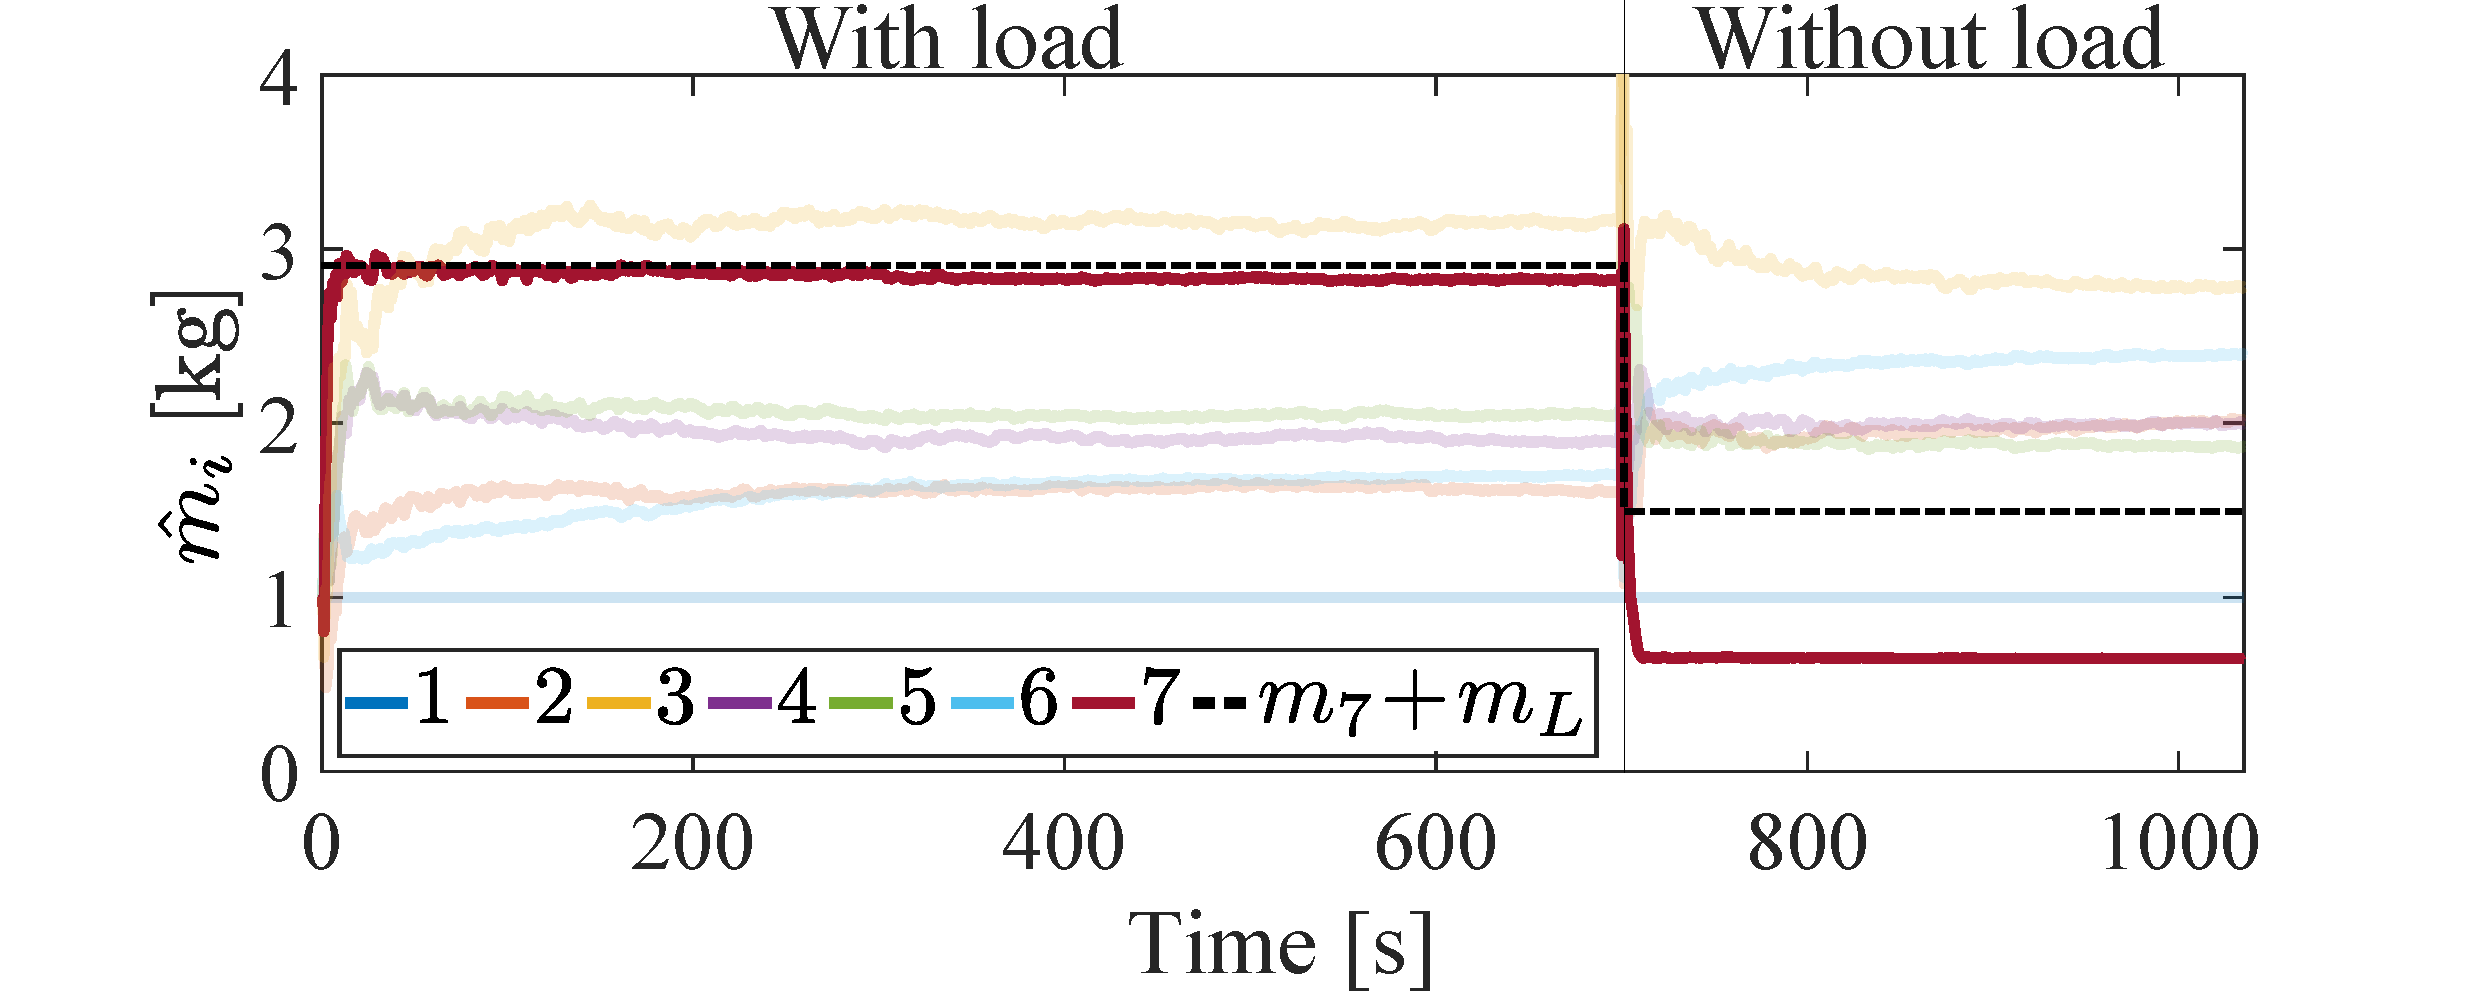
\includegraphics[width= 0.99\columnwidth]{fig/load_drop_mass_estimates_annotated_v3.pdf} 
%\hspace*{\fill}
%\caption[] {Relearning of the robot's link masses.}\label{fig:load_drop_mass_estimates}
%\end{figure}
%%---
%% ---------------------------------------------------------------------------------------------------
%\subsubsection{Comparison to a similar method}
%We implemented the natural adaptive controller (NAC) introduced in \cite{Lee2018naturaladaptivecontrol} to track the same excitation trajectory. In this method a Riemannian metric is used to derive a passibity-based parameter adaption law that uses natural gradient descent. This work directly compares to ours in that it deals with online estimation and physical feasibility. After a period of 1000 seconds the parameters were considered learned. Three aspects are of interest to us: the quality of the estimated parameters, their feasibility and the accuracy of the inverse dynamics torques that result from them. The former two points can be addressed by looking at the estimated mass and the eigenvalues of the density weighted covariance matrix for all links (i.e. $m_i$ and $ \lambda(\bm{\Sigma}_i) $) for methods RIL and NAC and comparing them against those from SID. In Table~\ref{tab:panda_simulation_results} we show the parameters grouped in the vector $ \bm{p}_i= [m, \lambda_1, \lambda_2, \lambda_3]^T  $ for all links for the three cases. Notice that feasibility is ensured as both, NAC and RIL, produced positive values. To evaluate the accuracy and generalizability of the inverse dynamics torques, we computed them for a new unseen trajectory using the (ground truth) parameters from SID and the estimated parameters from RIC and NAC and calculated the corresponding mean squared error,  $ J(\cdot) $, as defined in \eqref{eq:dyn_cost_func_euclidean}. Table~\ref{tab:panda_simulation_results} shows that $ J_{RIL} $  was orders of magnitude smaller than $ J_{NAC} $ at final time.
%%---
%\begin{table}[!t]
%\caption{Parameter feasibility and mean squared error for NAC and RIL relative to SID.}
%\centering
%\tiny
%\resizebox{\columnwidth}{!}{
%	\begin{tabular}{ p{0.05cm}p{0.2cm}p{0.3cm}p{0.3cm}p{0.3cm}p{0.3cm}p{0.3cm}p{0.3cm}p{0.3cm}p{0.5cm}}
%		\label{tab:panda_simulation_results}
%		& $\boldsymbol{p}$ & Link 1 & Link 2 & Link 3 & Link 4 & Link 5 & Link 6 & Link 7 & $J(\cdot)$\\    \hline
%		\multirow{4}{*}{\STAB{\rotatebox[origin=c]{90}{SID}}} & $m_i$	&	4.971	&	0.647	&	3.229	&	3.588	&	1.226	&	1.667	&	2.915	& \multirow{4}{*}{\STAB{\rotatebox[origin=c]{0}{N/A}}}\\
%		&$\lambda_{1}$	&	0.745	&	0.028	&	0.047	&	0.072	&	0.031	&	0.010	&	0.131 &	\\
%		&$\lambda_{2}$	&	0.006	&	0.003	&	0.016	&	0.012	&	0.010	&	0.002	&	0.018 &	\\
%		&$\lambda_{3}$	&	0.002	&	0.000	&	0.001	&	0.005	&	0.000	&	0.001	&	0.003 &	\\ \hline
%		\multirow{4}{*}{\STAB{\rotatebox[origin=c]{90}{NAC}}} & $m_i$	&	1.000	&	1.897	&	2.257	&	2.670	&	2.240	&	1.828	&	2.790	& \multirow{4}{*}{0.0037}\\
%		&$\lambda_{1}$	&	0.200	&	0.081	&	0.071	&	0.092	&	0.101	&	0.027	&	0.118 &	\\
%		&$\lambda_{2}$	&	0.015	&	0.021	&	0.019	&	0.013	&	0.007	&	0.007	&	0.010 &	\\
%		&$\lambda_{3}$	&	0.015	&	0.015	&	0.013	&	0.012	&	0.006	&	0.007	&	0.005 &	\\ \hline
%		\multirow{4}{*}{\STAB{\rotatebox[origin=c]{90}{RIL}}} & $m_i$	&	1.000	&	1.610	&	3.162	&	1.897	&	2.047	&	1.703	&	2.822 & \multirow{4}{*}{\textbf{9.7E-5}}	\\
%		& $\lambda_{1}$	&	1.000	&	0.073	&	0.048	&	0.121	&	0.098	&	0.025	&	0.120 &	\\
%		& $\lambda_{2}$	&	0.003	&	0.024	&	0.017	&	0.012	&	0.005	&	0.006	&	0.011 &	\\
%		& $\lambda_{3}$	&	0.003	&	0.009	&	0.006	&	0.008	&	0.003	&	0.005	&	0.003 &	\\
%		\hline
%\end{tabular}}
%\end{table}
%%---
%% ---------------------------------------------------------------------------------------------------
%\subsubsection{Comparison to neural networks}
%Today, neural networks (NN) are the flagship method for data-driven learning. For completeness, we briefly discuss the implementation of a simple NN to learn the inverse dynamics torque of the seventh links using the joint position, velocity and acceleration from all seven joints. A NN with two hidden layers, each having a 100 rectified linear units (ReLU), was used. We fed the NN the same 1000 seconds worth of data  seen by RIL and NAC as training data set and test for generalization on the same unseen trajectory. The results for the test, validation and training sets are shown in Table~\ref{tab:nn_results}. The results from the test set are far from satisfactory when compared to RIL on the same number of samples. Naturally, other architectures and networks (such as LSTMs \cite{Rueckert2017Learninginversedynamics} and recurrent NN \cite{Polydoros2017Onlinemultitarget}) could be used to learn inverse dynamics, but they always involve many hyperparameters and demand large amounts of data. Apart from this limitation, the lack of interpretability of the model is striking; e.g., the tested NN has 12,200 tunable parameters that provide no useful information about the system.
%%---
%\begin{table}[!t]
%\caption{Results using a neural network.}
%\vspace{-2ex}
%\begin{center}
%	\begin{tabular}[b]{p{1cm}p{1cm}p{1cm}} 
%		\hline
%		\textbf{$ J_{train} $} & $ J_{val} $ &  $ J_{test} $ \\ 			
%		\hline
%		0.042	  & 0.05 & 0.59\\
%		\hline
%	\end{tabular}
%\end{center}
%\label{tab:nn_results}
%\end{table}
%%---
%% SUBSECTION ========================================================================================
%\subsection{Test on a real Franka Emika Panda}
%We use RIL to learn the inertial parameters of a real Franka Emika Panda 7-DoF manipulator. Once again, the experiment consisted on the robot following repeatedly a precomputed 30 seconds excitation trajectory while holding an external load to excite the torques at the distal joints. The robot was driven by a built-in velocity tracking controller. Measurement data from the robot was recorded at a rate of 1 kHz and included joint angle and torque. Joint velocity was obtained using numerical differentiation. As for joint acceleration, since there is no direct measurement for it, the desired values were taken instead under the assumption that the controller achieves a small tracking error (i.e. $ \ddot{\bm{q}} \approx \ddot{\bm{q}}_{ref}$). Since we \textbf{do not} make assumptions about the inertial properties of the links \textbf{nor} have any initial values taken from a CAD software or any other source, we select once again the initial guess $ \hat{\bm{P}}_0 $ as an identity matrix for all links. Regarding RAMSGrad hyperparameters, we took the defaults values for $ \beta_1 = 0.9 $ and $ \beta_2 = 0.999 $ and settled for a learning rate $ \alpha = 0.01 $. Since we focus on trying to find the parameters of the robot, we provide information to the algorithm about the inertial properties of the load. 
%
%% SUBSECTION ========================================================================================
%\subsubsection{Impact of noise}\label{sec:results}
%%\textcolor{red}{We observed that RAMSGrad was particularly sensitive to noise as it hindered parameter convergence introducing high variability in the updates. To combat this we increased the size of the replay buffer and the mini batches to $N_{\mathcal{B}} = 10000$ and $N_{\mathcal{X}} = 5$. With this strategy it was possible to shrink the parameter update variability and elucidate a convergence trend. Fig.~\ref{fig:results_panda} shows this trend in the parameters of interest to evaluate physical feasibility (an exponential moving average was superimposed on the plots to facilitate readability); i.e. mass and eigenvalues of the density weighted covariance matrix $ \bm{\Sigma} $. As all values are positive at all times, then \emph{feasibility is ensured}.	As for the learned inertia ellipsoids, similar to the case study, the distal-most links were better estimated, with the proximal links suffering from identifiability limitations and lack of excitation.}
%\textcolor{black}{We observed that RAMSGrad was particularly sensitive to noise as it hindered parameter convergence introducing high variability in the updates. To combat this we increased the size of the replay buffer to $N_{\mathcal{B}} = 10000$ keeping the mini batch size as $N_{\mathcal{X}} = 5$. With this strategy it was possible to shrink the parameter update variability and reveal a convergence trend.}
%% ---------------------------------------------------------------------------------------------------
%\subsubsection{Comparison to system identification}
%Figs.~\ref{fig:panda_ril_parameters} and \ref{fig:panda_sid_parameters} report the full set of inertial parameters obtained from RIL and SID. Although we cannot fully learn the parameters of proximal links since it is a fixed-base robot, RIL was able to learn a more consistent description of the second link, as the mass found in  SID  is comparatively too small (considering that the first two links are structurally similar). The remaining masses are comparable in both methods. As for the remaining parameters, a qualitative assessment can be made by looking at the resulting inertial ellipsoids shown in Figs.~\ref{fig:panda_ril_parameters} and \ref{fig:panda_sid_parameters}. The distal-most links were better estimated, with the proximal links suffering from identifiability limitations and lack of excitation. While both sets satisfy full physical feasibility, there are differences in how well the ellipsoids represent their corresponding link. For instance, as joint motors represent a large part of the link mass, it is expected that the center of mass will be close to the joint location\footnote{Please note that the method followed in \cite{Gaz2019Dynamicidentificationfranka} considered a numerical model of the robot manipulator available from the robot interface, thus, additional information that is not available in our online learning setting.}. Looking at the inertia ellipsoids, it seems that RIL learns a better representation of the inertial parameters of the distal-most links (links 5-7), based on their orientation and center point location. In contrast, the parameters for links 3 and 4 obtained from the system identification process are more consistent (both ellipsoids are comparable in size, as expected from the actual shape of the links). Finally, estimation of the proximal links was unsatisfactory as both methods struggle to generate a good representation for the first link, even though RIL was able to learn a more reasonable mass for link 2. 
%%---
%\begin{figure}[!t]
%\begin{tabular}{m{1.5cm} m{3cm}}
%	\centering
%	\tiny
%	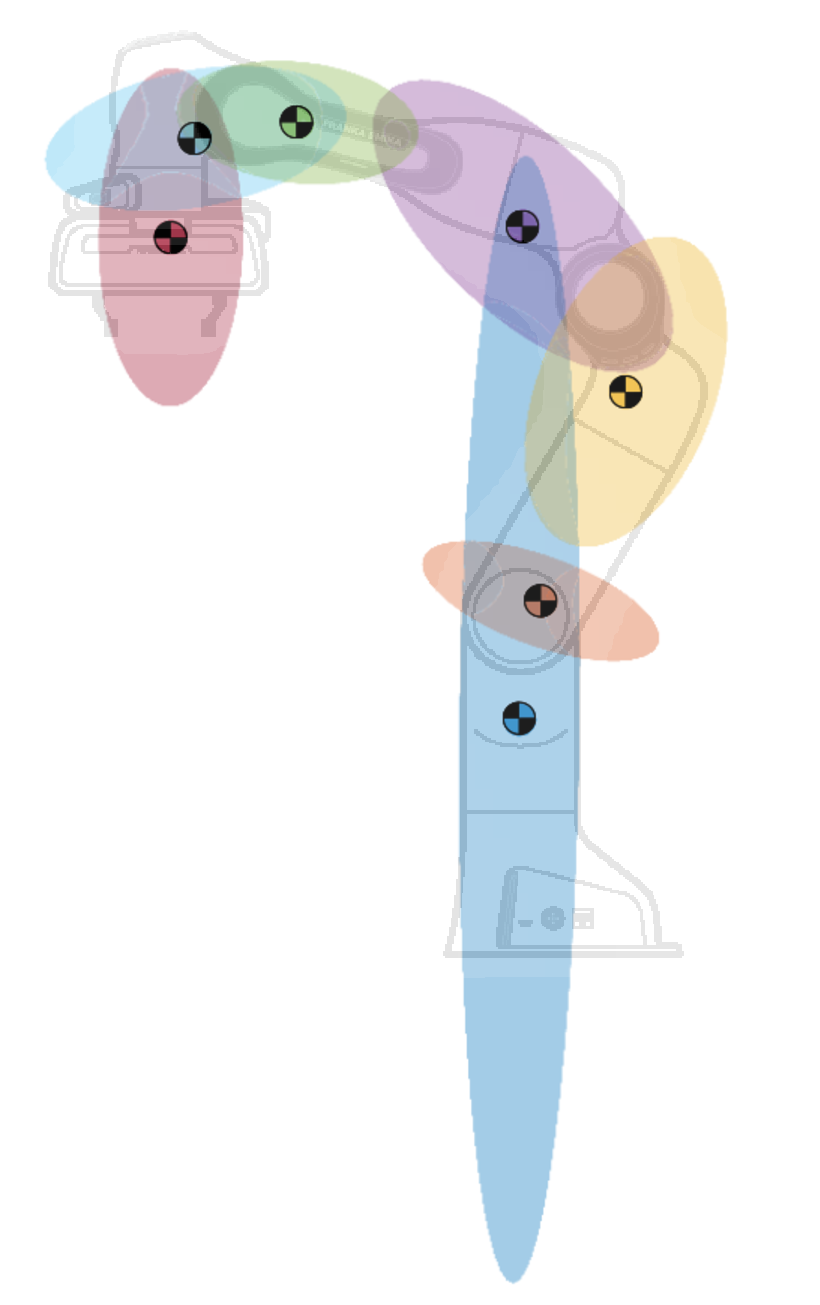
\includegraphics[width = 0.25\columnwidth]{fig/panda_ellipsoid_estimates_sid.pdf} 
%	&
%	\resizebox{0.75\columnwidth}{!}{
%		\begingroup
%		\setlength{\tabcolsep}{1pt} % Default value: 6pt
%		%\renewcommand{\arraystretch}{1.5} % Default value: 1
%		\tiny
%		\begin{tabular}[b]{p{0.6cm}p{0.6cm}p{0.6cm}p{0.6cm}p{0.6cm}p{0.6cm}p{0.6cm}p{0.6cm}}
%			$\boldsymbol{\theta}$ & Link 1 & Link 2 & Link 3 & Link 4 & Link 5 & Link 6 & Link 7\\    \hline
%			$m_i$	&	4.9707	&	0.6469	&	3.2286	&	3.5879	&	1.2259	&	1.6666	&	1.4655	\\
%			$m_iX_{i}$	&	0.0193	&	-0.0020	&	0.0888	&	-0.1908	&	-0.0147	&	0.1002	&	0.0004	\\
%			$m_iY_{i}$	&	0.0103	&	-0.0186	&	0.1267	&	0.3746	&	0.0503	&	-0.0235	&	-0.0031	\\
%			$m_iX_{i}$	&	-0.4654	&	0.0023	&	-0.2147	&	0.0985	&	-0.0471	&	-0.0175	&	0.1453	\\
%			$XX_i$	&	0.7470	&	0.0085	&	0.0565	&	0.0677	&	0.0394	&	0.0025	&	0.0308	\\
%			$XY_i$	&	-0.0002	&	-0.0040	&	-0.0082	&	0.0277	&	-0.0015	&	0.0015	&	0.0004	\\
%			$XZ_i$	&	0.0086	&	0.0103	&	-0.0055	&	0.0039	&	-0.0046	&	-0.0001	&	-0.0007	\\
%			$YY_i$	&	0.7503	&	0.0281	&	0.0529	&	0.0324	&	0.0315	&	0.0106	&	0.0284	\\
%			$YZ_i$	&	0.0201	&	0.0008	&	-0.0044	&	-0.0016	&	0.0022	&	0.0001	&	-0.0005	\\
%			$ZZ_i$	&	0.0092	&	0.0265	&	0.0182	&	0.0776	&	0.0109	&	0.0118	&	0.0067	\\
%			\hline
%		\end{tabular}
%		\endgroup
%	}
%\end{tabular}
%\caption{Inertial parameters and ellipsoids from SID.}\label{fig:panda_ril_parameters}
%\end{figure}
%%---
%\begin{figure}[!t]
%\begin{tabular}{m{1.5cm} m{3cm}}
%	\centering
%	\tiny
%	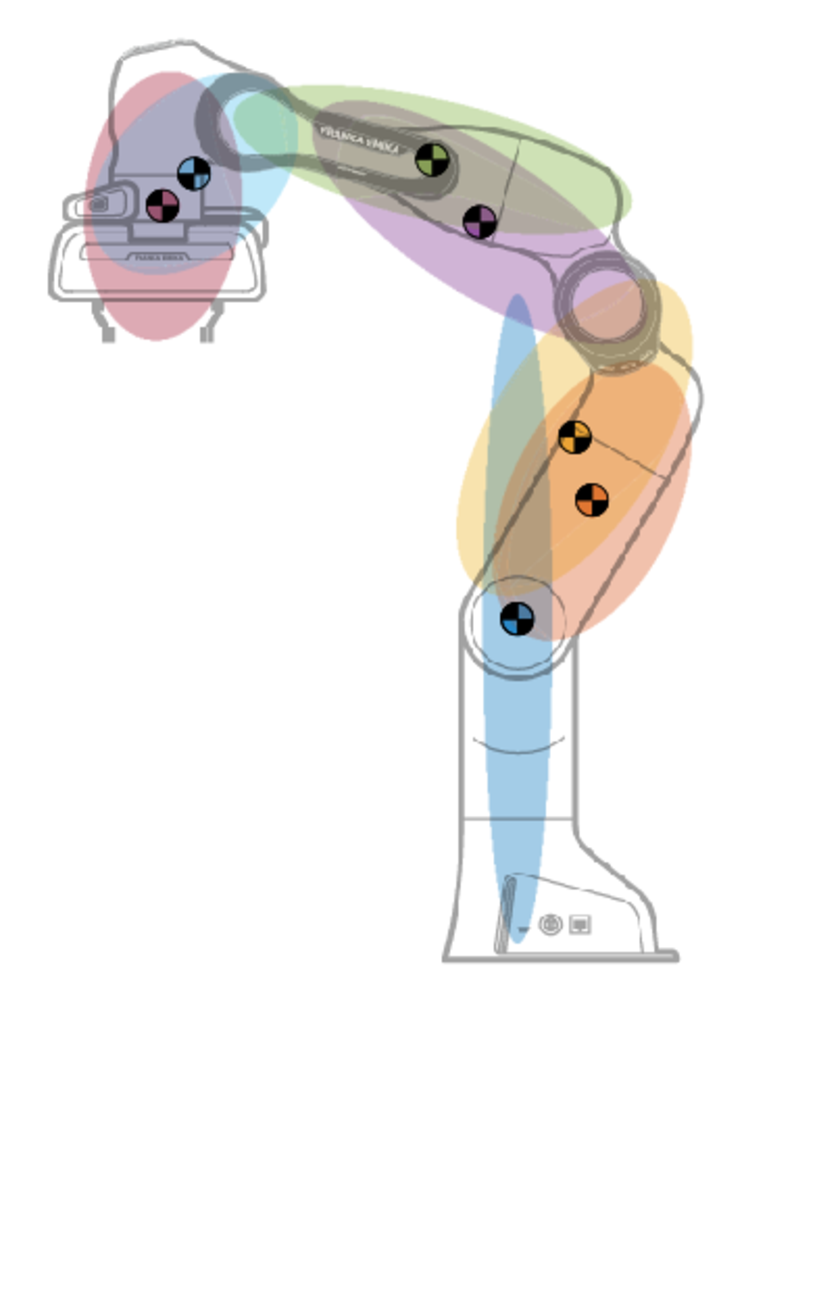
\includegraphics[width= 0.25\columnwidth]{fig/panda_ellipsoid_estimates_ril.pdf} 
%	&
%	\resizebox{0.75\columnwidth}{!}{
%		\begingroup
%		\setlength{\tabcolsep}{1pt} % Default value: 6pt
%		%\renewcommand{\arraystretch}{1.5} % Default value: 1
%		\tiny
%		\begin{tabular}[b]{p{0.6cm}p{0.6cm}p{0.6cm}p{0.6cm}p{0.6cm}p{0.6cm}p{0.6cm}p{0.6cm}}
%			$\boldsymbol{\theta}$ & Link 1 & Link 2 & Link 3 & Link 4 & Link 5 & Link 6 & Link 7\\    \hline
%			$m_i$	&	1.000	&	2.6473	&	3.1301	&	2.4053	&	1.8933	&	1.9949	&	1.4170	\\
%			$m_iX_{i}$	&	0.000	&	-0.0143	&	0.1289	&	-0.1090	&	-0.0209	&	0.1173	&	0.0013	\\
%			$m_iY_{i}$	&	0.000	&	-0.3686	&	-0.0052	&	0.3392	&	0.0289	&	-0.1009	&	0.0139	\\
%			$m_iX_{i}$	&	0.000	&	0.0673	&	-0.4106	&	-0.0002	&	-0.3443	&	-0.0451	&	0.0774	\\
%			$XX_i$	&	1.006	&	0.0998	&	0.1051	&	0.1067	&	0.1078	&	0.0182	&	0.0161	\\
%			$XY_i$	&	0.000	&	0.0049	&	0.0000	&	0.0300	&	0.0003	&	0.0066	&	-0.0001	\\
%			$XZ_i$	&	0.000	&	-0.0029	&	0.0018	&	0.0000	&	-0.0035	&	0.0030	&	-0.0028	\\
%			$YY_i$	&	1.006	&	0.0348	&	0.1179	&	0.0250	&	0.1065	&	0.0190	&	0.0183	\\
%			$YZ_i$	&	0.000	&	0.0161	&	-0.0031	&	-0.0022	&	0.0044	&	-0.0022	&	-0.0006	\\
%			$ZZ_i$	&	0.012	&	0.1020	&	0.0249	&	0.1169	&	0.0099	&	0.0243	&	0.0099	\\
%			\hline
%		\end{tabular}
%		\endgroup
%	}
%\end{tabular}
%\caption{Inertial parameters and ellipsoids from RIL.}\label{fig:panda_sid_parameters}
%\end{figure}
%%---
%% ---------------------------------------------------------------------------------------------------
%\subsubsection{Inverse dynamics estimation}\label{sec:inv_dyn_estimation}
%%---
%\begin{figure*}[t!]
%\centering
%\hspace*{\fill}
%\subfloat[]{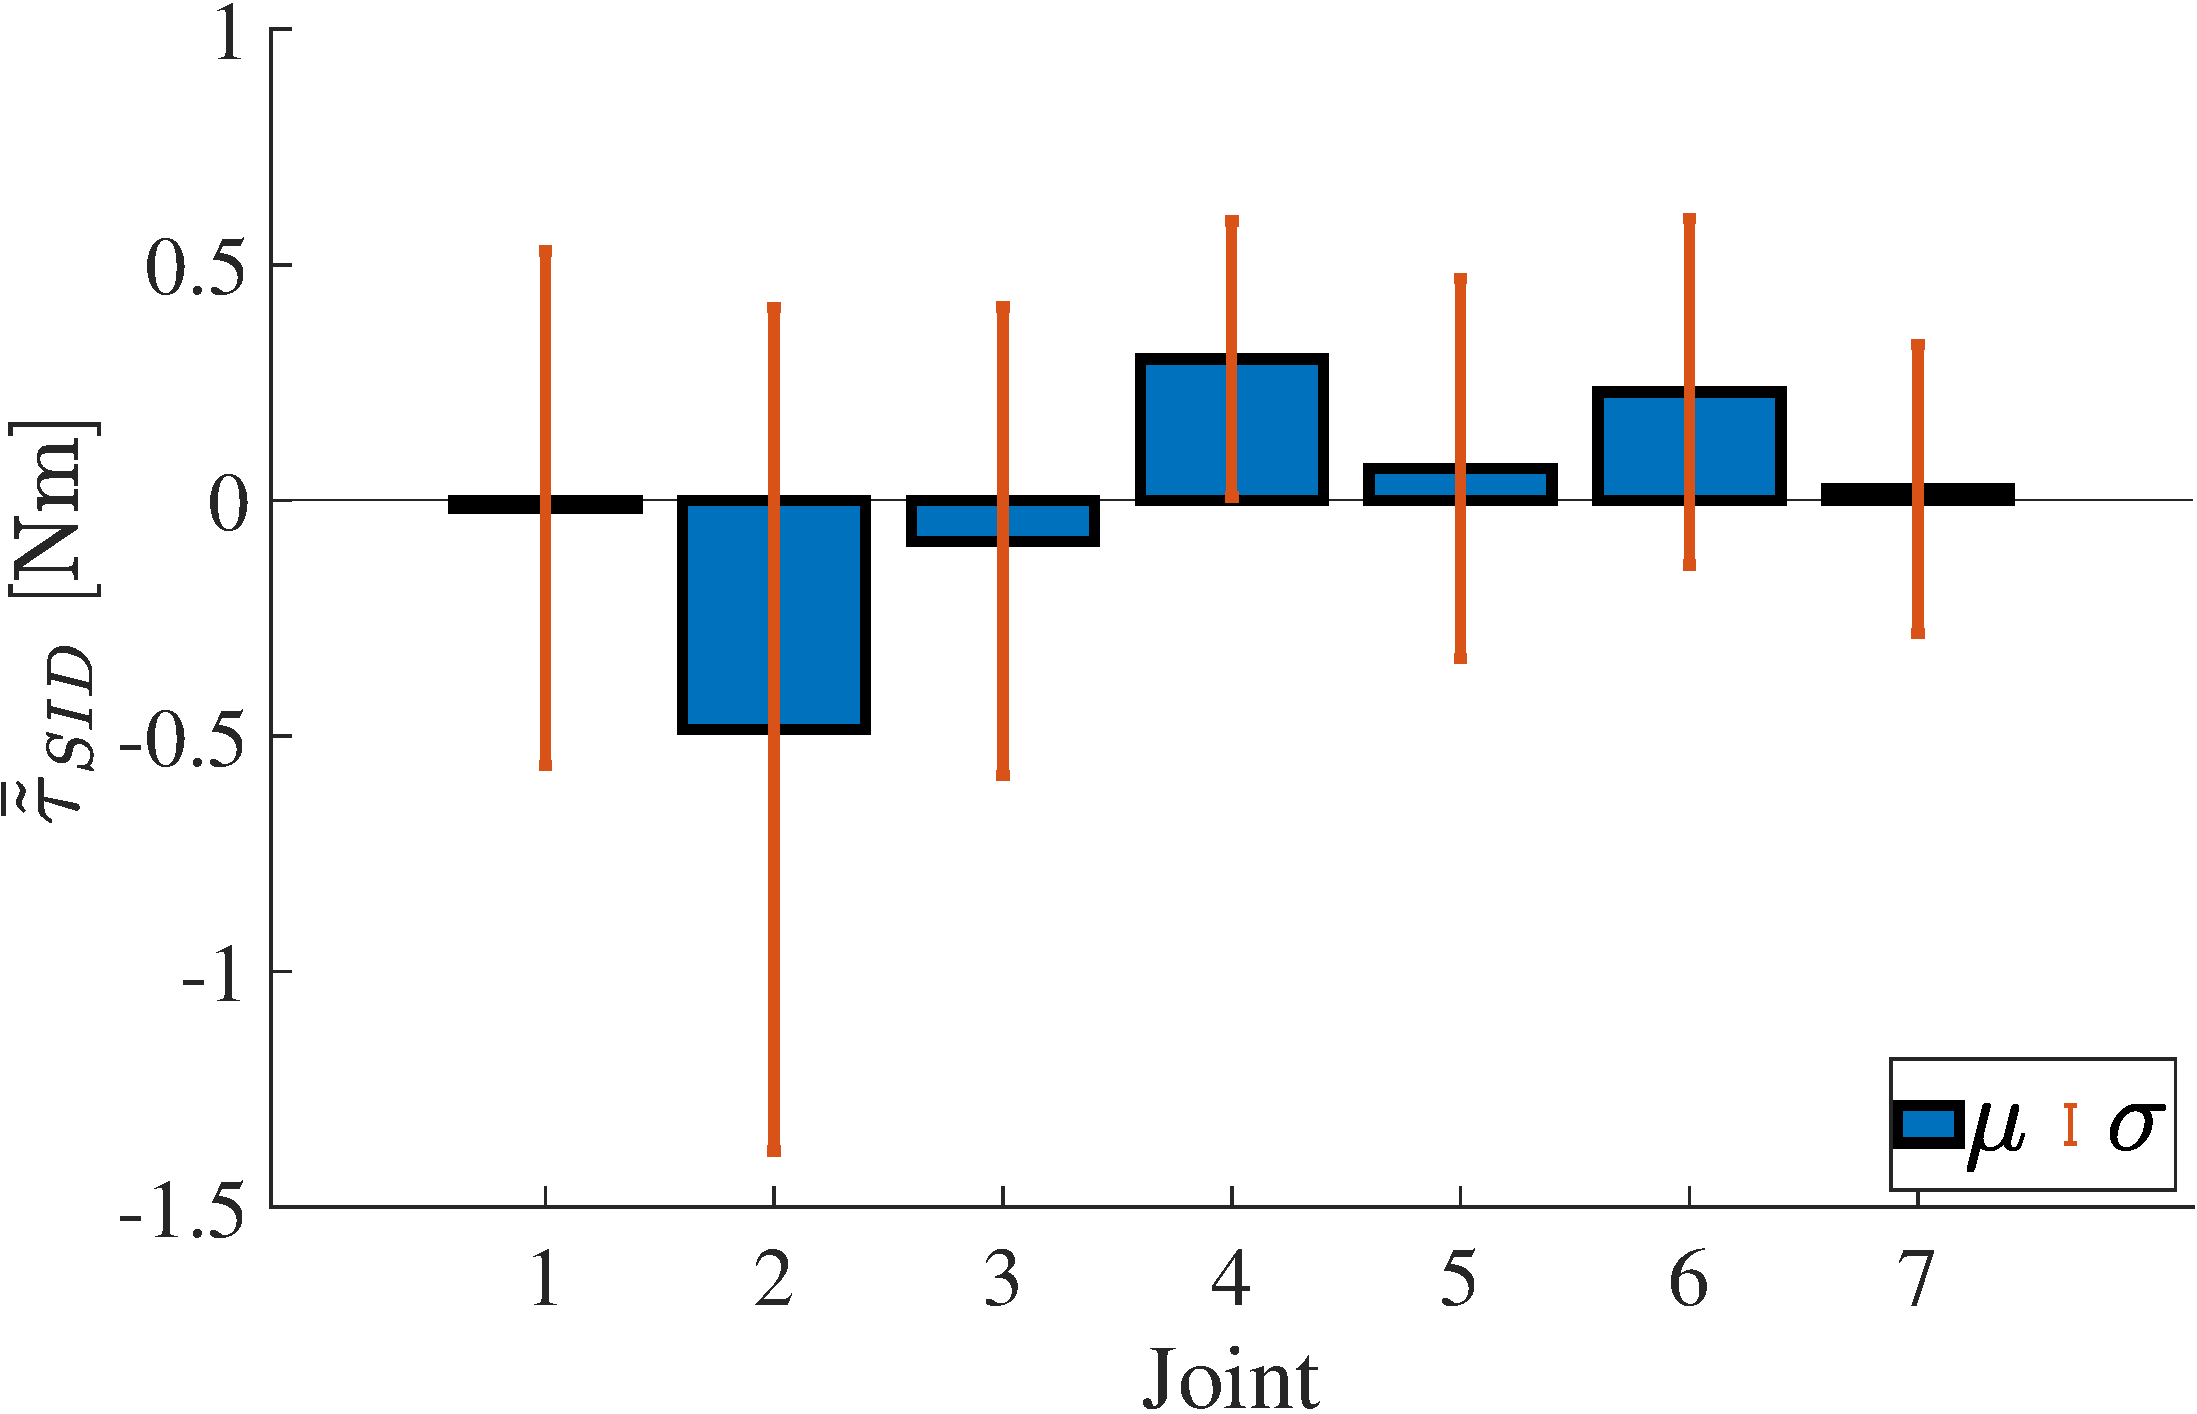
\includegraphics[width= 0.23\textwidth]{fig/panda_torque_sid_abs_error.pdf} \label{fig:panda_torque_error_sid_statistics}}
%\hspace{-0.2em}
%\subfloat[]{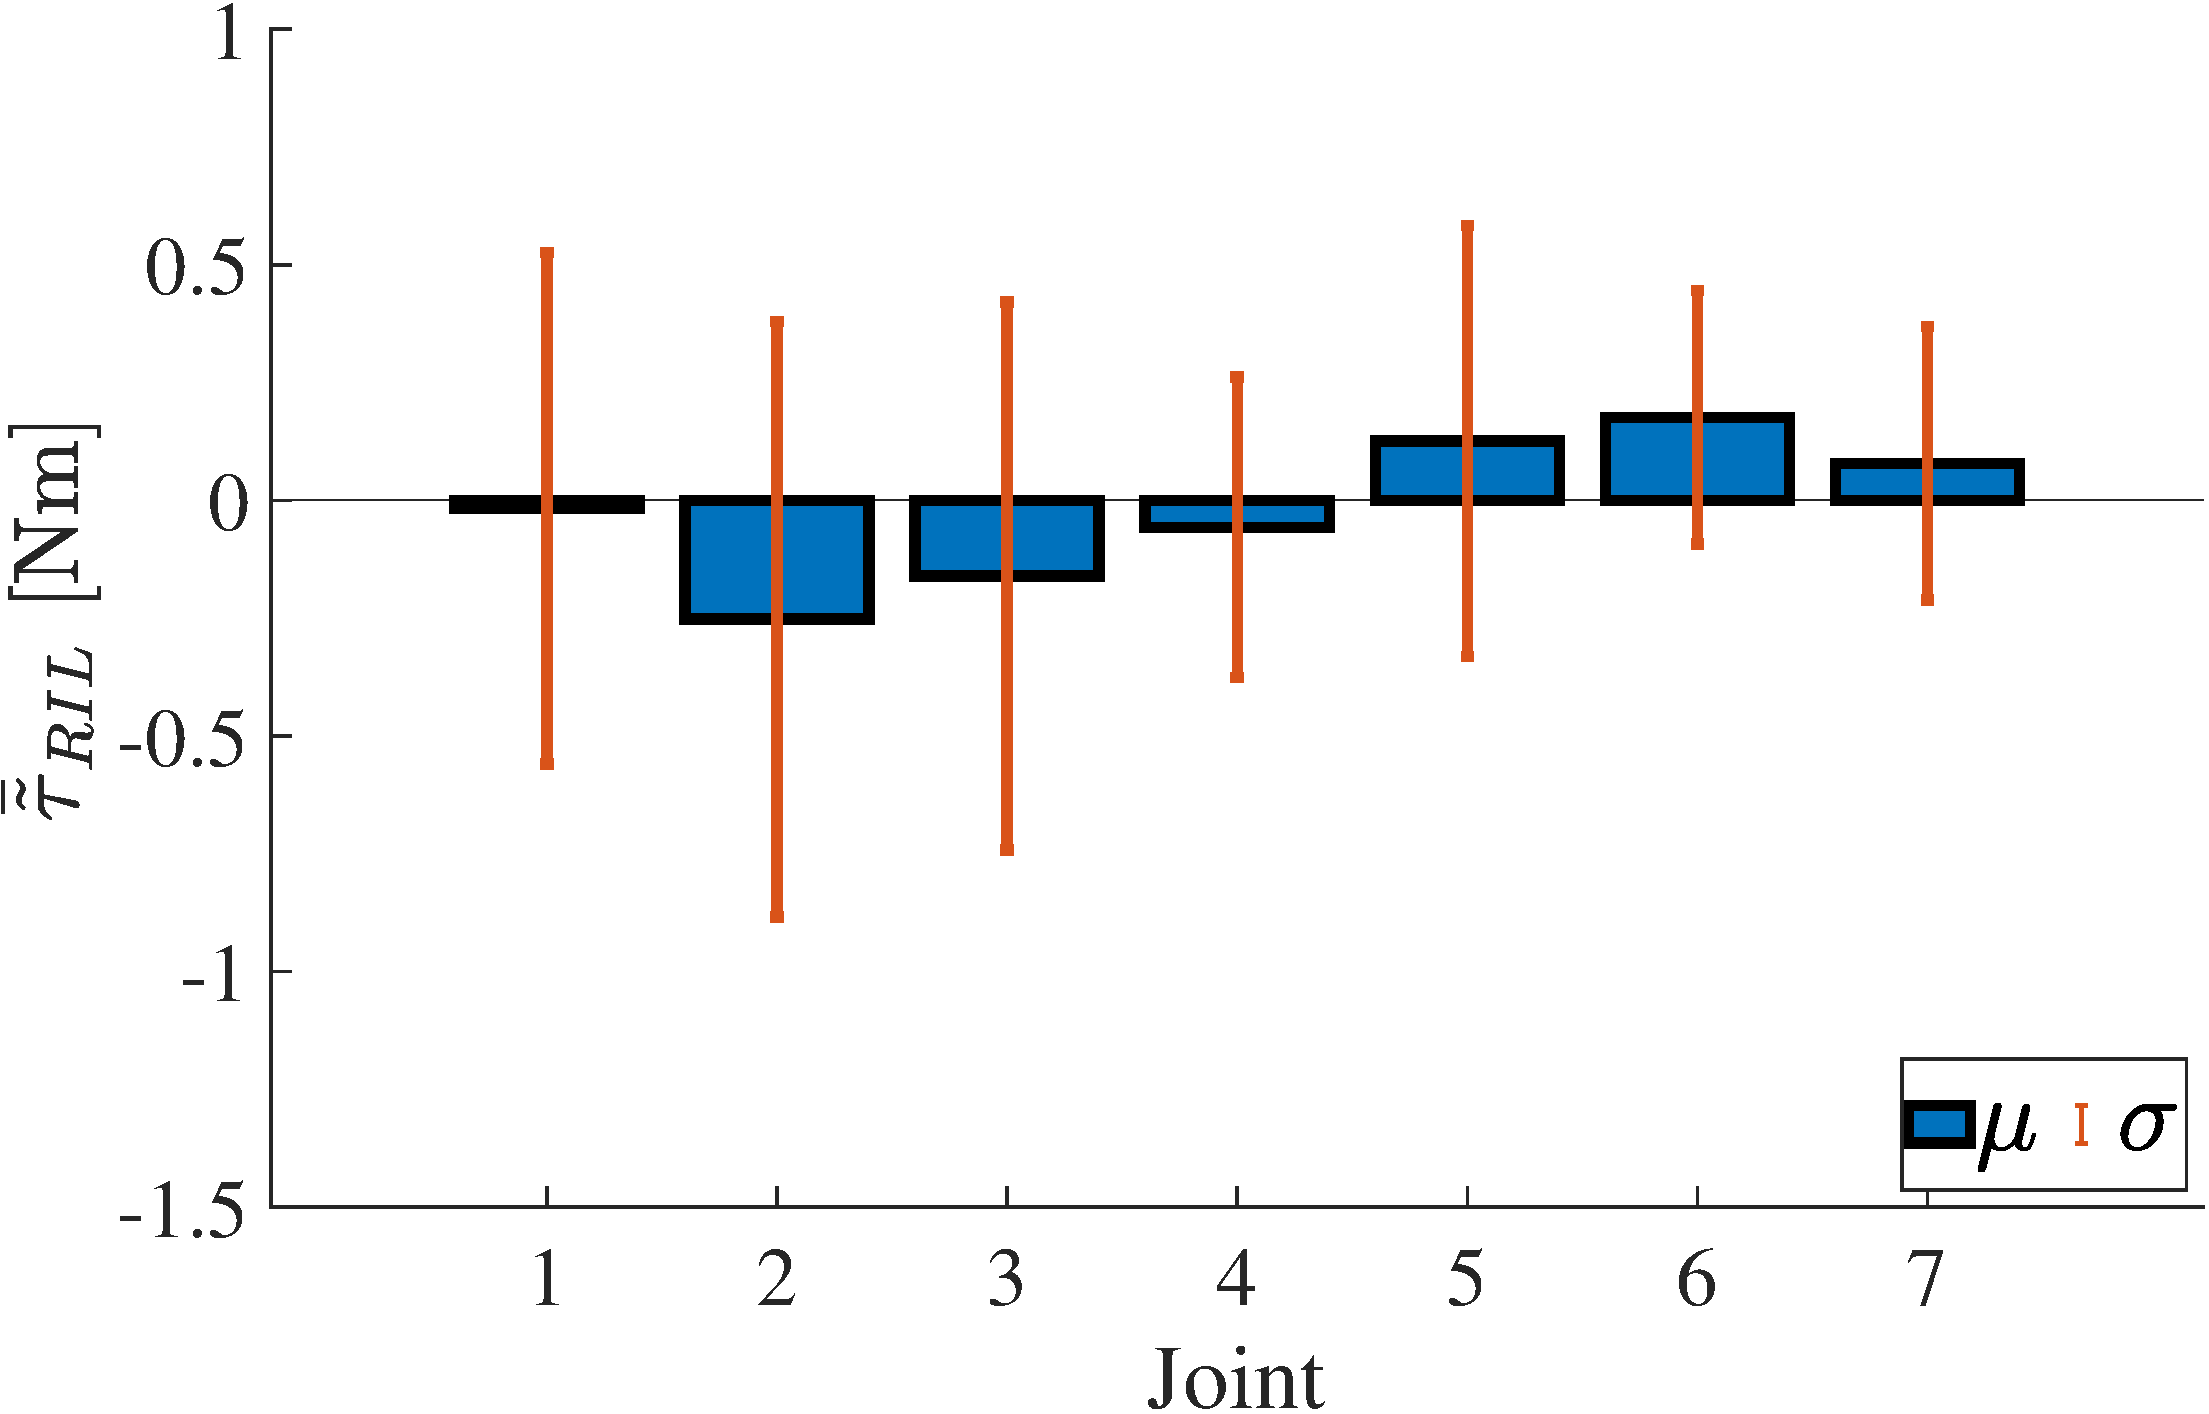
\includegraphics[width= 0.23\textwidth]{fig/panda_torque_ril_abs_error.pdf} \label{fig:panda_torque_error_ril_statistics}}			
%\hspace{-0.2em}
%\subfloat[]{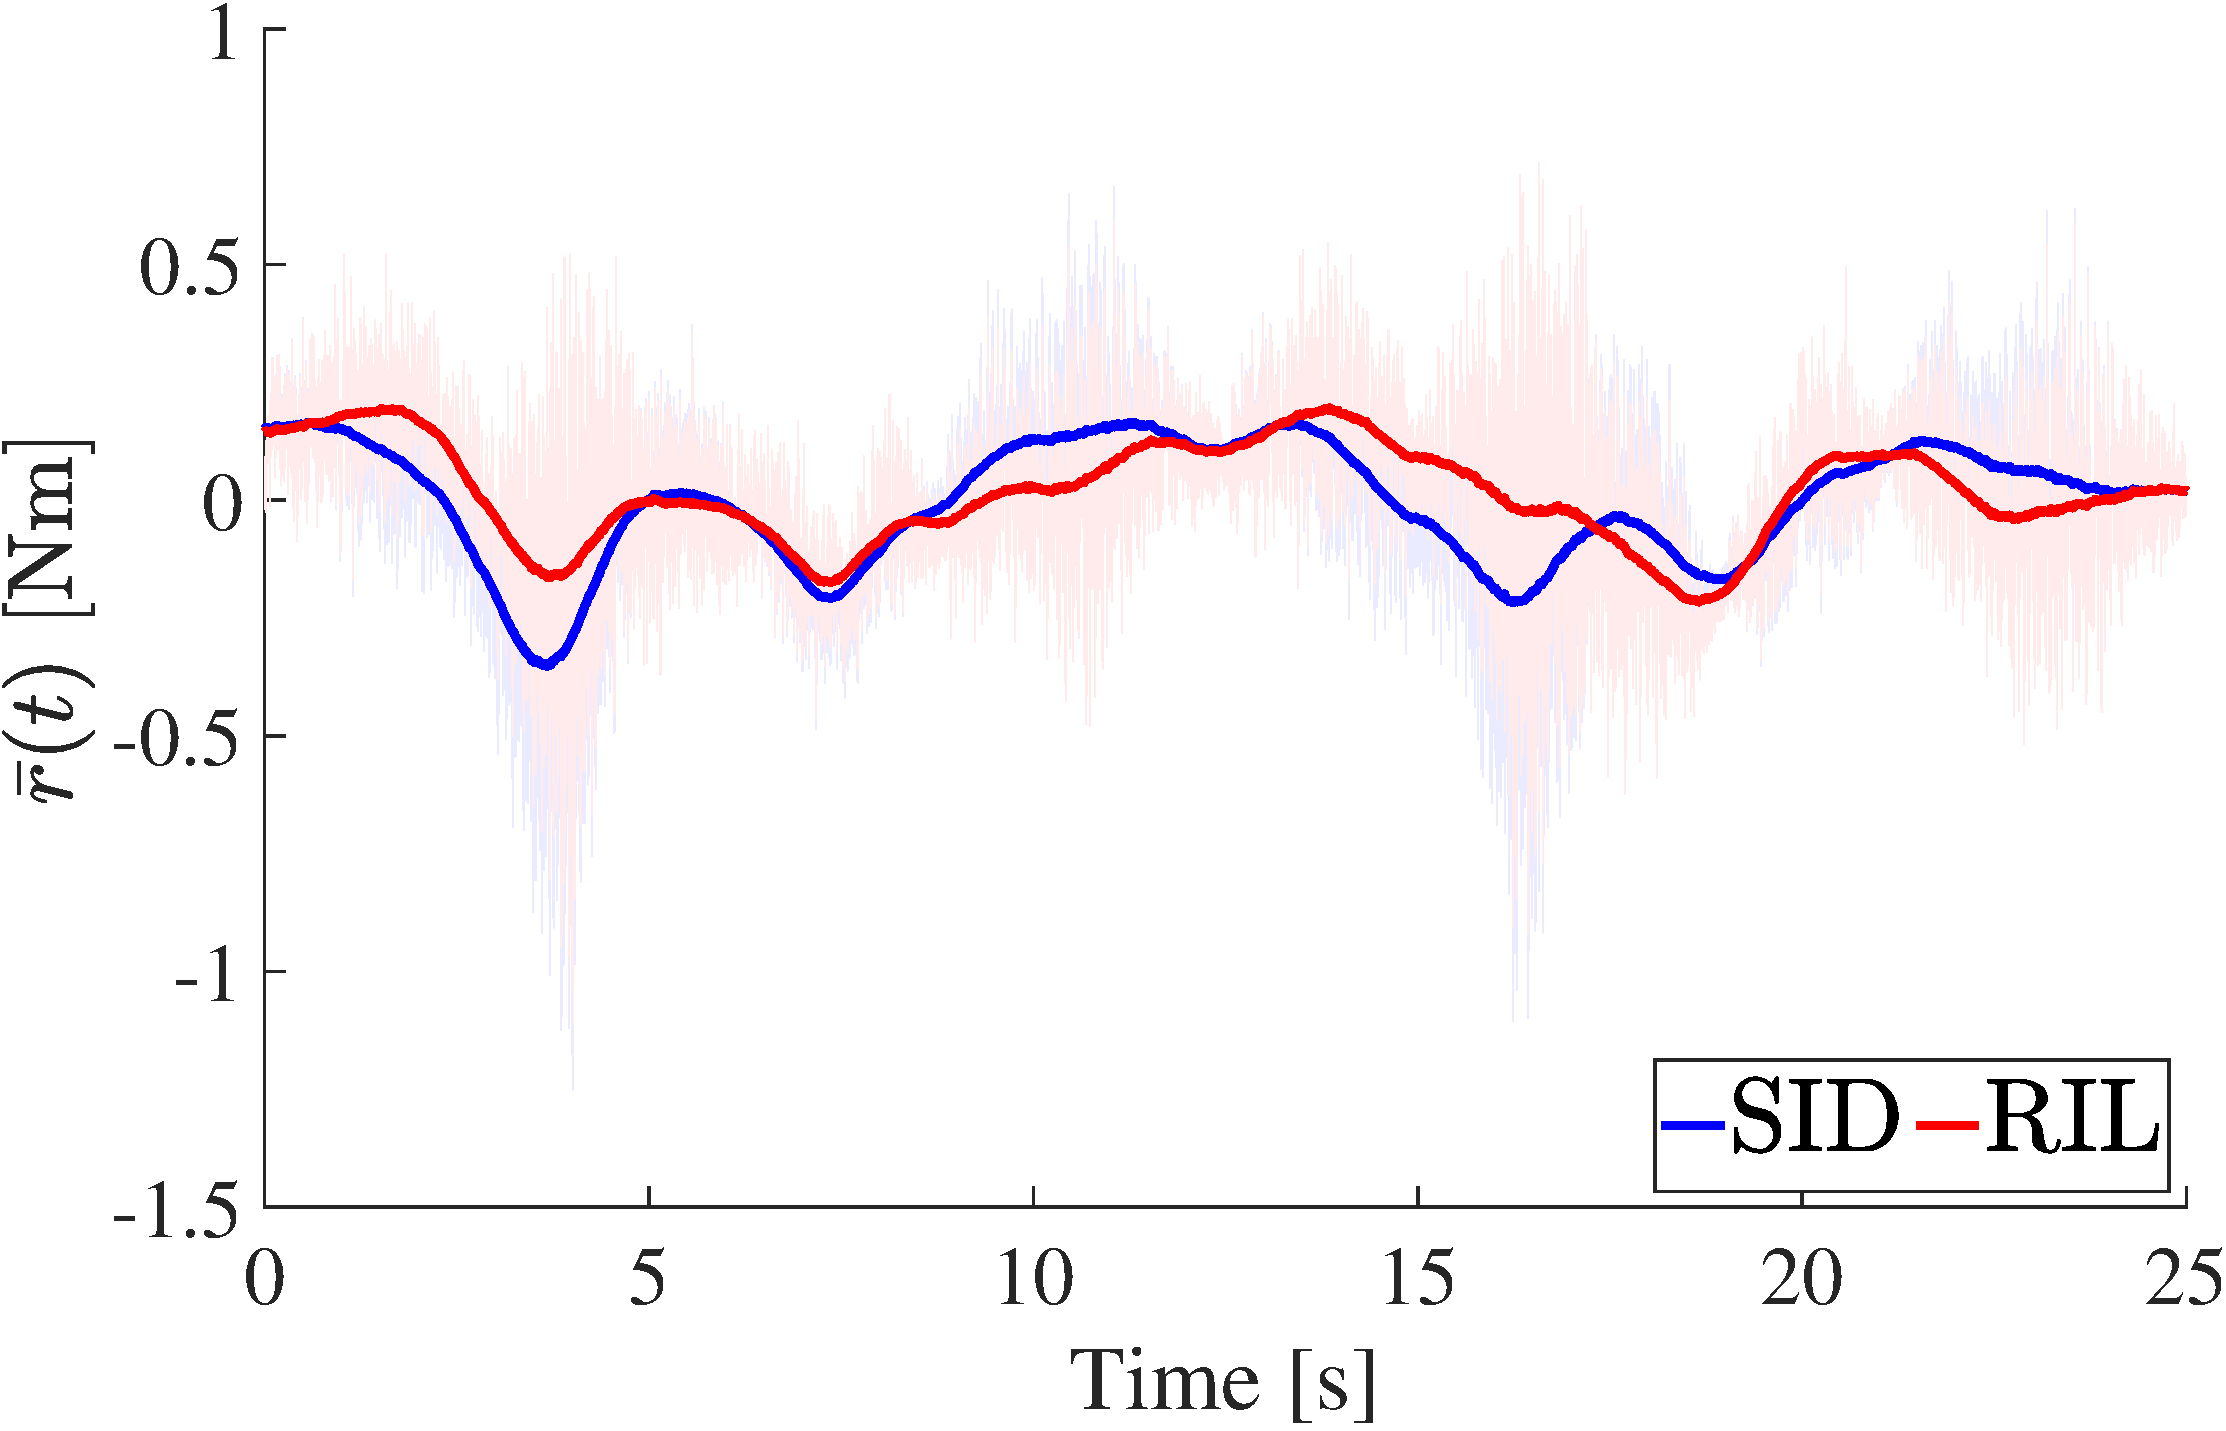
\includegraphics[width= 0.23\textwidth]{fig/momentum_residual_average.pdf} \label{fig:momentum_residual_average}}	
%\hspace{-0.2em}
%\subfloat[]{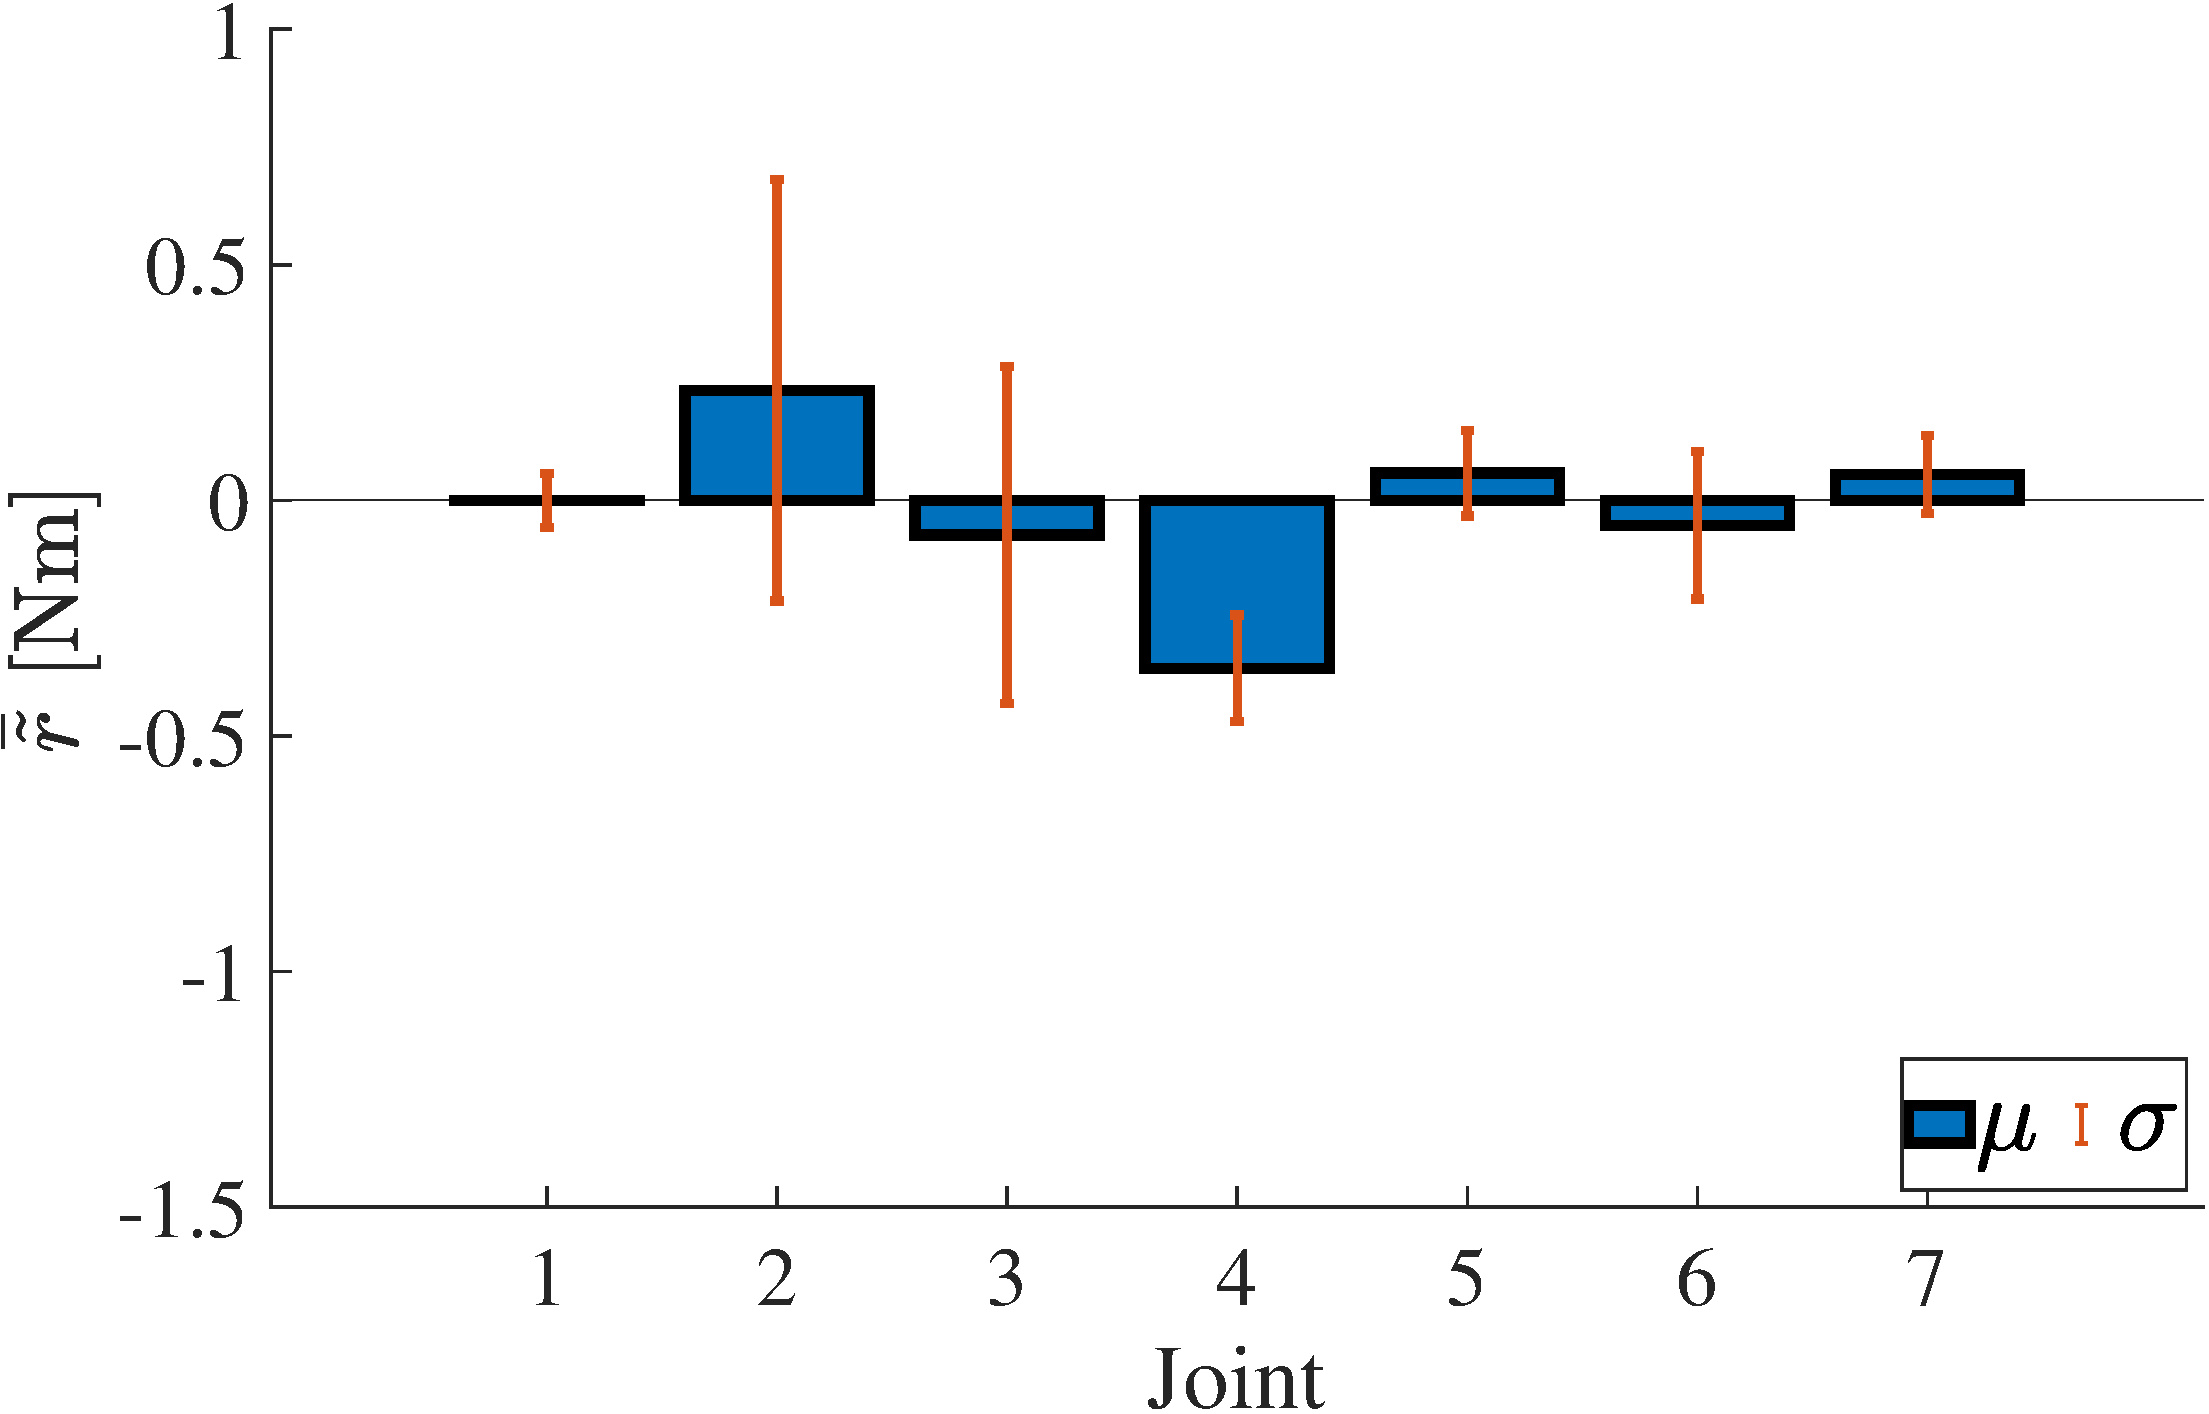
\includegraphics[width= 0.23\textwidth]{fig/residual_abs_error.pdf} \label{fig:residual_abs_error}}			
%\hspace*{\fill}
%\caption[] {\label{fig:panda_inverse_dynamics_torque_estimation} Experimental results: average absolute error for \subref{fig:panda_torque_error_sid_statistics} SID and \subref{fig:panda_torque_error_ril_statistics} RIL, \subref{fig:momentum_residual_average} momentum average residual and \subref{fig:residual_abs_error} average absolute residual per joint.}
%\end{figure*}
%%---
%A goal of characterizing the inertial properties of the robot's body schema is to use it as an inverse dynamics model. Consequently, we assess here the accuracy of the inverse dynamics torques $ \hat{\bm{\tau}} $ that result from $ \hat{\bm{\theta}} $. For a different 25 seconds trajectory we: record its joint torques $ \bm{\tau} $, compute the corresponding torque estimates, and obtain the estimation error $ \tilde{\bm{\tau}}_{RIL} = \bm{\tau} - \hat{\bm{\tau}}_{RIL} $. The mean $ \mu $ and standard deviation $ \sigma $ of its value for all joints during the experiment is shown in Fig.~\ref{fig:panda_torque_error_ril_statistics}. Observe that estimation for the large torques in proximal joints was rather good. In contrast, the error was more apparent in distal joints, where torques had smaller magnitudes. Nonetheless, the generated inverse dynamics torque closely reproduce the measured ones. Moreover, it could be further improved as the robot keeps collecting more diverse data samples during operation. Additionally, we computed the SID inverse dynamics torques (denoted here by $ \tilde{\bm{\tau}}_{SID} = \bm{\tau} - \bm{\tau}_{SID} $). Notoriously, the torques are practically the same and the errors can be attributed to minor non modeled effects and observed noise ($\pm$\SI{0.5}{\newton\meter} in the measured torque signal).
%
%% SUBSECTION ========================================================================================
%\subsection{A measure of model quality}
%The parameter estimates $ \hat{\bm{\theta}} $ can be used to reconstruct the standard rigid body dynamics model of the robot, i.e.
%\begin{equation}\label{eq:robt_dynamics_eq}
%\hat{M}(\bm{q};\hat{\bm{\theta}})\ddot{\bm{q}} + \hat{c}(\bm{q},\dot{\bm{q}};\hat{\bm{\theta}})+ \hat{g}(\bm{q};\hat{\bm{\theta}}) = \bm{\tau}_m + \bm{\tau}_{ext} - \bm{\tau}_{\epsilon}
%\end{equation}
%with $ \hat{M} $ being the robot mass matrix, $ \hat{\bm{c}} $ is the vector of centrifugal and Coriolis forces and $ \hat{\bm{g}} $ is the gravity torque vector. The RHS of \eqref{eq:robt_dynamics_eq} includes the motor, external and modeling error torques, respectively. 
%
%To provide further insight into the quality of a given set of learned inertial parameters, we used a momentum observer \cite{Haddadin2017Robotcollisionssurvey} whose output is given by:
%%---
%\begin{align}
%\bm{r}(t) &= \bm{K}\left(\bm{p}(t) - \int_{0}^{t}\left(\bm{\tau}_m - \hat{\bm{g}} - \hat{c}  \dot{\hat{\bm{M}}}+ \bm{r} \right)ds - \bm{p}(0)\right)\label{eq:observer_residual}
%\end{align}
%%---
%where $ \bm{p}=\hat{\bm{M}}(\bm{q})\dot{\bm{q}} $ is the generalized momentum estimate, $ \bm{K} $ is a diagonal matrix of positive values and $ \bm{r} $ is the monitoring residual. As the observer depends on an estimated model, then $ \bm{r} $ would converge to zero only if a perfect model is available and if no external torque is acting on the robot (i.e. $ \bm{\tau}_{ext}=0 $). Assuming the latter, then, by differentiating \eqref{eq:observer_residual} we obtain the residual dynamics $ \dot{\bm{r}}=-\bm{K}\left(\bm{\tau}_\epsilon + \bm{r}\right) $, whose solution converges asymptotically to $ \bm{\tau}_\epsilon $. We ran the momentum observer on the test trajectory and used two models: (a) one from $ \hat{\bm{\theta}}_{SID} $ and (b) $ \hat{\bm{\theta}}_{RIL} $. Fig.~\ref{fig:momentum_residual_average} shows the average of the residuals $ \bar{\bm{r}} $ for all seven joints for SID and RIL, where clearly $ \bar{\bm{r}}_{SID} \approx \bar{\bm{r}}_{RIL} $ . In Fig.~\ref{fig:residual_abs_error} we show the mean and standard deviation for the difference of the residuals of each joint $ \tilde{r}_i $; where it is apparent that the differences are negligible.
%
%% SUBSECTION ========================================================================================
%\subsection{Discussion}\label{sec:discussion}
%RIL comes with a few challenges. First, parameter convergence is slower than conventional euclidean unconstrained methods. Second, due to manifold operators, generating Riemannian updates is computationally more demanding. Third, RAMSGrad seems to be more sensitive to the learning rate $\alpha$ than its Euclidean homologue, which can be attributed to the curvature of $ \mathcal{M} $. Fourth, the algorithm's performance was hindered by measurement noise. Despite these challenges, RIL presents interesting areas of opportunity. For instance, although we used the standard values for the decay rates $ \beta_1 $ and $ \beta_2 $ further research can determine more appropriate values which can eventually cope with the learning rate challenge. Likewise a better use of the replay buffer $ \mathcal{B} $ and the mini batches $\mathcal{X}$ together with a more computationally efficient implementation can help leveraging past information to get a better parameter convergence and reduce the impact of noise. Furthermore, as discovering the body schema is in itself a self-driven task, developing a reward-based online motion strategy that induces efficient self exploration of the state space can contribute to a faster learning of the inertial parameters. A key point is that, unlike other algorithms, we do not need here any  previous knowledge to determine the initial guess, requiring only that $\hat{\bm{P}}_0 \in \mathcal{S}^4_{++}$. Additionally, the observed experimental inverse dynamics errors are comparable with those obtained by other offline methods using full data batches (e.g. see results in \cite{Sousa2019Inertiatensorproperties, Wensing2017Linearmatrixinequalities}) but with the added benefit of online learning. Moreover, from the relatively small values in the residual differences and inverse dynamics torques we can conclude that the model from RIL is qualitatively comparable to that from SID. Finally, there is the most appealing benefit: full physical feasibility at every time step. This guarantees valid incrementally-learned parameters that generate accurate inverse dynamics torques and can be used in other model-based techniques.
%
%% ===================================================================================================
%%                                                 |                                                 |
%%                                                 |                                                 |
%% -------------------------------------------- SECTION ---------------------------------------------|
%%                                                 |                                                 |
%%                                                 |                                                 |
%% ===================================================================================================
%\section{Conclusions}\label{sec:conclusion}
%We introduced the RIL method to characterize the dynamical properties of a robot's body schema. 
%Analysis on a virtual manipulator confirmed that RIL provides guarantees on the physical feasibility and learns consistent parameters at all times without prior information. Although experiments on a real robot exhibited high sensitivity to noise, the experience replay buffer helped to obtain parameter updates with reduced variability. Analysis of the inverse dynamics torques and modeling errors indicate that RIL is able to produce valid sets of inertial parameters that can generate accurate inverse dynamic torques and that result in consistent models. RIL opens pathways towards adaptable models that respect physical constraints, thus, positively impacting control and safety applications where failing to provide valid parameters may induce instabilities. Finally, we see potential in the method to be naturally complemented with a learning scheme that computes excitation motions online.